
\chapter{Hose-Drum-Unit Control}

Aerial refueling (AR) is an effective method of increasing the endurance and
range of aircraft by refueling them in flight \cite{AAR-2014},
\cite{luo2019docking}. Among the aerial refueling methods in operation today,
the probe-drogue refueling (PDR) \cite{bhandari2013bow} is the most widely
adopted one owing to its flexibility and simple requirement for equipment. In
this chapter, the low-level flight control for PDR is focused, where the
station-keeping control and the docking control are included. First,
the station-keeping control is the basis of autonomous aerial refueling. However,
there exist strong external disturbances including the atmospheric turbulence
and the wake vortex of the tanker, and the system perturbation caused by the fuel
transfer. These pose challenges to station-keeping control design. This
chapter proposes an additive-state-decomposition-based (or state-compensation-linearization-based) station-keeping control
method for autonomous aerial refueling. Moverover, designing a controller for
the docking maneuver in PDR is the most important but challenging task, due to
the complex system model and the high precision requirement. In order to
overcome the disadvantage of only feedback control, a additive-state-decomposition-based feedforward control
scheme known as iterative learning control (ILC) proposed in \textit{Chapter 6} is adopted here.

\section{Introduction}

Autonomous Aerial Refueling (AAR) is an effective method of increasing
the endurance and range of Unmanned Aerial Vehicles (UAVs) \cite{lee2017optimal,olavo2018robust,roberge2018fast}
by refueling them in flight \cite{Thomas2014}. The Probe-and-Drogue
Refueling (PDR) is widely adopted in AAR owing to its simple requirement
of equipment and flexibility. In a PDR system, there is a hose payout
and reel-in device which is called Hose-Drum Unit (HDU) \cite{Ro2011}
(also known as the reel take-up system \cite{Vassberg2003,vassberg2005numerical}).
It consists of a hose-drum motor and a motor control unit, and determines
the motion of the upper end of the hose \cite{Ro2011}. It is an important
device to suppress the hose whipping phenomenon (HWP), which can result
in severe damage to the probe or the drogue \cite{Wang2014}.

The HWP is caused by the excessive contact between the probe and the
drogue. The existing literature focused on how to design an HDU controller
to maintain the tension of the hose and suppress HWP, such as \cite{Vassberg2003,Wang2014}.
In practice, the drogue will remain relatively static if the hose-drogue
system is not affected by wind disturbances. In this situation, the
\textquotedblleft excessive contact\textquotedblright{} is hard to
happen because tracking a static target is a relatively easy and simple
task. However, when affected by wind disturbances, the drogue is always
moving, so the receiver has to speed up to chase the drogue which
may result in excessive contact and HWP. In addition to suppressing
the HWP after the contact, this chapter tries to reveal that the HDU
can also be applied as a feedback damper to reduce the frequency and
amplitude of the drogue position fluctuation under wind disturbances,
which has not attracted enough attention in the previous research.
Fortunately, the basic models were established by the existing literature,
which can be employed to analyze the dynamics of the drogue with HDU
controller. The hose-drogue dynamic model is established and the behavior
of the drogue in the docking stage is analyzed by references \cite{Ro2011,Vassberg2003,vassberg2005numerical,Ro2009,Zhu2006}.

In the whole refueling process, the motion of the drogue is influenced
by many types of wind disturbances, such as the aerodynamic influence
of the tanker \cite{Yue2016}, atmospheric turbulence \cite{Chen2007},
the bow wave effect \cite{Dibley2007PhaseI}, and so on. According
to the NASA flight test results \cite{Dibley2007PhaseI} as shown
in Fig.\,\ref{F_Wei_2015}(a), the drogue fluctuates with the amplitude
about 0.1$\sim$0.2m (mainly caused by atmospheric turbulence, and
the amplitude depends on the weather condition) in a low frequency
when the receiver is far away. When the receiver comes close to the
drogue, the drogue is quickly pushed away by the bow wave flow field
with offset about 0.4m (dotted ellipse region in Fig.\,\ref{F_Wei_2015}(a)),
and this docking attempt is failed because the probe is too slow to
chase the drogue. As a result, in the docking stage, the bow wave
of the receiver is the most substantial one. Thus, the hose-drogue
model under the bow wave is simplified by reference \cite{Wei2015,Dai2015},
which is called the drogue dynamic model. Moreover, the motion of
the drogue under the bow wave and its control methods are studied
in \cite{dai2018terminal,dai2018iterative,ren2019Reliable}. However,
there were some differences (the dotted ellipse regions in Fig.\,\ref{F_Wei_2015})
between the simulation results generated by the drogue dynamic model
(see Fig.\,\ref{F_Wei_2015}(b)) and the flight test experiment (see
Fig.\,\ref{F_Wei_2015}(a)) \cite{Dibley2007PhaseI}, where the simulation
results are about 40\% larger than the experimental results, especially
for the vertical position. One of the main reasons is that the effects
of HDU were not considered by the drogue dynamic model. Thus, the
results of reference \cite{Wei2015} are improved in this chapter by
considering the effects of HDU. Meanwhile, the traditional HDU control
methods mainly feedback the hose tension to reduce the drogue fluctuation
and suppress HWP to some extent, but it cannot avoid HWP essentially
because it cannot detect whether the HWP is happening and its degree.
Since the HWP is essentially caused by the over-slack of the hose
due to excessive contact on the drogue, this chapter proposed an anti-HWP
control method to monitor the state of the hose and control the hose
length to stabilize the drogue movement.

In summary, the main contributions of this chapter are: (i) a more precise
modeling method for hose-and-drogue system is proposed based on the
previous study; (ii) by considering the effects of HDU controller,
an improved integrated model is proposed to describe more accurately
the behavior of the drogue under wind disturbances, and a simplified
drogue dynamic model is obtained through system identification for
the convenience of docking controller design of the receiver aircraft;
(iii) improvements are proposed for the traditional HDU controllers
to realize a better performance to stabilize the drogue position under
disturbances before the contact happens; (iv) for the excessive contact
situations, an anti-HWP control method is proposed to significantly
reduce the effect of hose whipping phenomenon and improve the safety
of aerial refueling systems.

\begin{figure}[ptb]
	\begin{centering}
		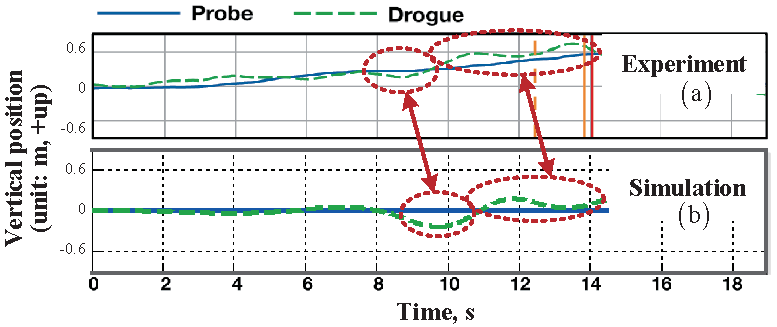
\includegraphics[width=0.48\textwidth]{Figures/Figs_Ch8/Fig01} 
		\par\end{centering}
	\caption{The vertical motion of the drogue in reference \protect \cite{Wei2015}}
	\label{F_Wei_2015} 
\end{figure}

This chapter is organized as follows. Section II describes the drogue dynamic model with HDU and demonstrates the procedure of researching the effects of HDU. Section III compares two types of controllers for HDU, and the corresponding drogue dynamic models with HDU controllers are obtained by following the procedure of the simulation as mentioned in Section II. Their performances are also compared in this section. The anti-HWP control method is proposed and verified in Section IV. Finally, the conclusions are given in Section V.

\section{Drogue Dynamic Model with HDU}
The HDU is situated within the refueling pod, as shown in Fig. \ref{F_HDU_POD}. It primarily consists of a drum (reel) that winds the hose, a motor responsible for controlling the rotation of the drum, and a controller for the motor. The rotation of the motor is primarily controlled based on the status of the upper end of the hose connected to the refueling pod. This device regulates the hose tension by adjusting the length of the hose exposed outside when the hose tension is insufficient. It effectively mitigates the phenomenon of hose whipping by reducing the risk of sudden tension changes, thereby minimizing potential refueling accidents caused by such effects.
\begin{figure}[th]
	\centering
	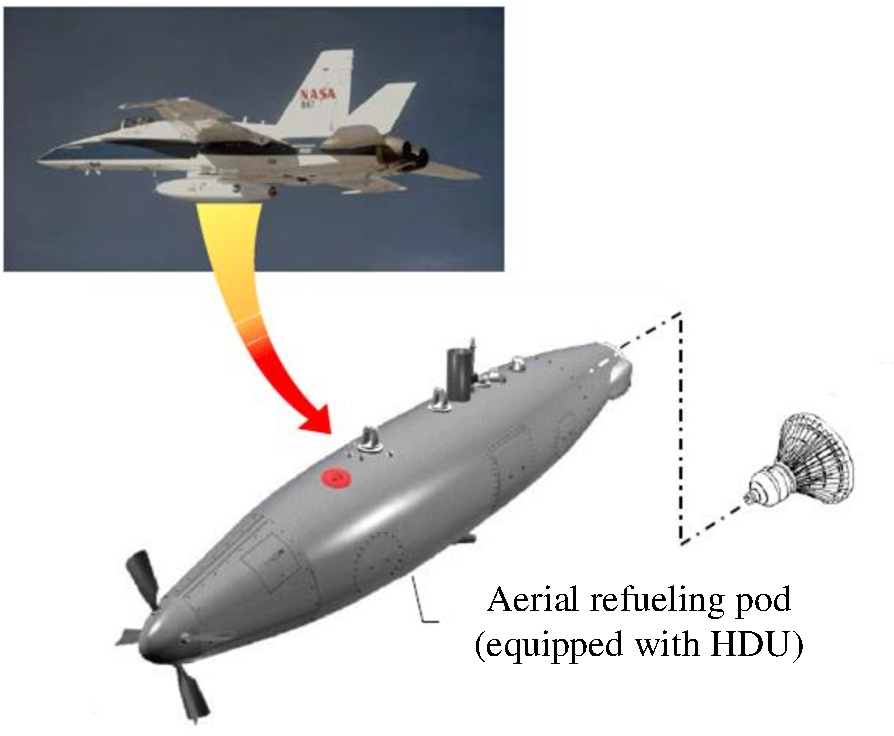
\includegraphics[width=0.6\textwidth]{Figures/Figs_Ch8/Fig04}
	\caption{Refueling Pod and HDU Schematic}\label{F_HDU_POD}
\end{figure}
Currently, research on the HDU primarily focuses on designing controllers to regulate the hose tension and suppress hose whipping phenomenon. Hose whipping usually occurs after the docking of the drogue and probe, but the HDU's role in suppressing hose whipping also affects the dynamics of the hose-drogue assembly during the docking process. However, this aspect has received relatively little attention in current research. Therefore, this section will provide an initial analysis of this impact.

\subsection{Analysis of Fixed-Length link-connected model Deficiencies}

Based on the analysis in Section 4.3.4, the significant downward movement of the drogue in the ${o_{\rm{t}}}{z_{\rm{t}}}$ direction compared to the experiment can be observed. From this phenomenon and the corresponding time of occurrence, it can be inferred that this dynamic motion of the drogue in the ${o_{\rm{t}}}{z_{\rm{t}}}$ direction is caused by the component of the bow wave in the ${o_{\rm{t}}}{x_{\rm{t}}}$ direction, meaning that the force in the ${o_{\rm{t}}}{x_{\rm{t}}}$ direction induces a substantial displacement of the drogue in the ${o_{\rm{t}}}{z_{\rm{t}}}$ direction. The reason behind this phenomenon is that the hose-drogue system is under tension when in a steady state, making the hose behave more rigidly. The hose-drogue system is approximately similar to a simple pendulum near its equilibrium position \cite{williamson_controllable_2010}, as depicted in Fig. \ref{F_Pendulum}.

\begin{figure}[ptb]
	\begin{centering}
		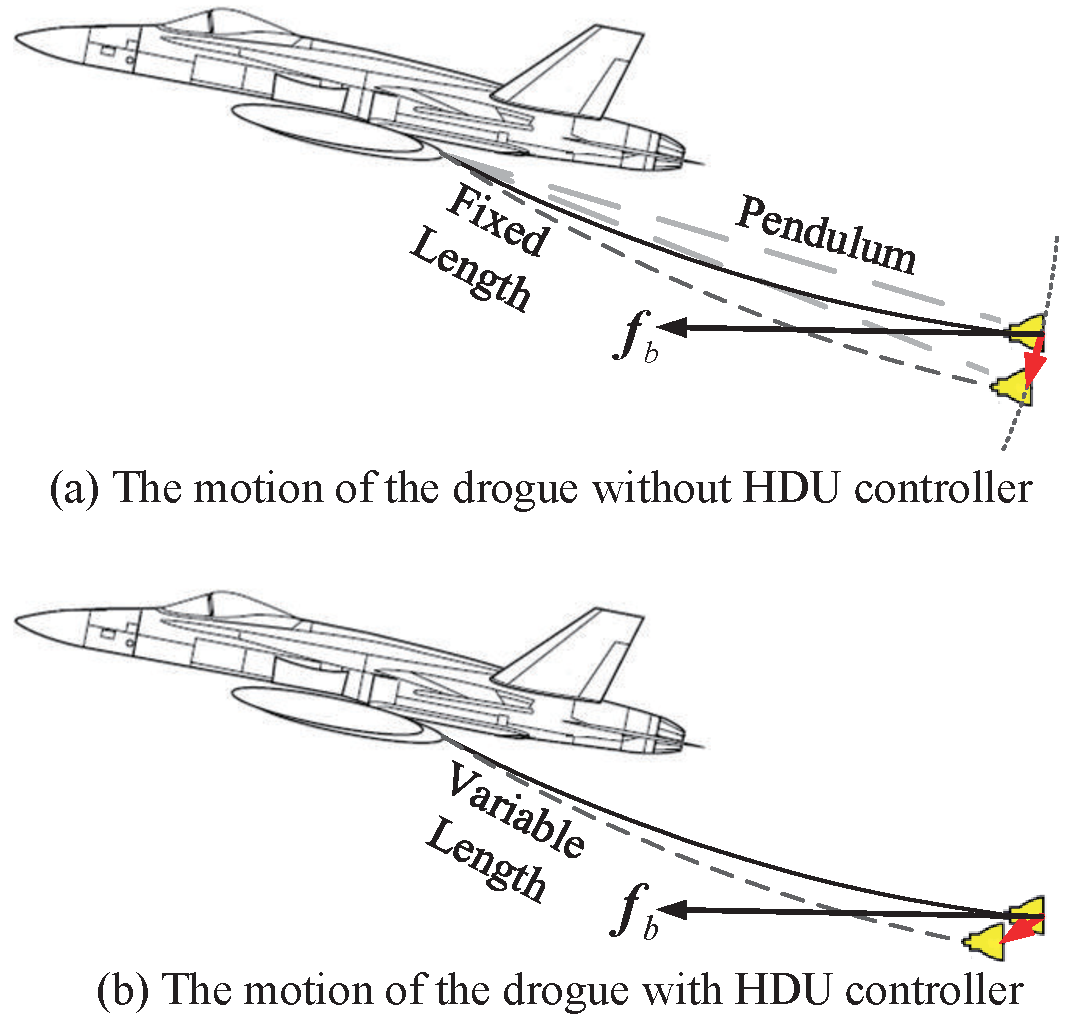
\includegraphics[width=0.48\textwidth]{Figures/Figs_Ch8/Fig03}
		\par\end{centering}
	\caption{The motion of the drogue with and without HDU controller}
	\label{F_Pendulum} 
\end{figure}

In the absence of the HDU, the pendulum length remains unchanged, as shown in Fig. \ref{F_Pendulum}(a). Within the equilibrium range, applying a force to the endpoint of the pendulum, apart from the force direction normal to the equilibrium position, will result in a tangential motion of the pendulum due to forces acting in other directions. In a steady state, the hose tends to be in a more horizontal position, causing both ${F_{{\rm{b}}x}}$ and ${F_{{\rm{b}}z}}$ to primarily induce displacement of the drogue along the ${o_{\rm{t}}}{z_{\rm{t}}}$ direction. This also indicates a significant coupling of the drogue's dynamics in the absence of the HDU.
When the HDU is considered, it adjusts the length of the exposed hose outside the aircraft in response to changes in hose tension, as depicted in Fig. \ref{F_Pendulum}(b). When the drogue experiences a longitudinal force ${F_{{\rm{b}}x}}$ from the bow wave, the HDU reduces the length of the exposed hose, thereby changing the primary direction of movement of the drogue from downward to forward. It is evident that the HDU modifies the dynamics of the drogue during the docking process.

\subsection{Model of the HDU}

The model of the HDU typically employs a reel model\cite{vassberg_numerical_2004}, and its dynamics can be expressed as follows 
\begin{equation}\label{E_ModelHDU}
\left( {{T_{{\rm{reel}}}} - {T_{{\rm{hose}}}}} \right){r_{{\rm{reel}}}} = {I_{{\rm{reel}}}}{\alpha _{{\rm{reel}}}}
\end{equation}
where ${T_{{\rm{reel}}}}$ and ${T_{{\rm{hose}}}}$ represent the tension in the reel and the tension at the upper end of the hose, respectively. Since the direction of force is not analyzed here, scalar magnitudes of tension are used. The symbols ${r_{{\rm{reel}}}}, {I_{{\rm{reel}}}}$ and ${\alpha _{{\rm{reel}}}}$ represent the radius of the reel, moment of inertia, and angular acceleration around its central axis. Furthermore, if the reel is considered as a cylindrical object, one have 
\begin{equation}\label{eq4.119}
{I_{{\rm{reel}}}} = {m_{{\rm{reel}}}}r_{{\rm{reel}}}^2\text{.}
\end{equation}
On the other hand, expressing ${\alpha _{{\rm{reel}}}}$ in terms of linear acceleration 
\begin{equation}\label{eq4.120}
{\alpha _{{\rm{reel}}}} = \frac{{{{\ddot l}_1}}}{{{r_{{\rm{reel}}}}}}\text{.}
\end{equation}
It should be noted that the change in the length of the hose is replaced by the change in the length of the first link. Although from Section 4.2 it can be understood that the one exposed is the $i$th link, due to the relatively small retraction of the hose during the docking process, extending the original length of the first link appropriately ensures that the first link is always exposed. Of course, the model of variable first link in Section 4.2.5 can also be used, but it involves more complex calculations. Substituting Eqs. (\ref{eq4.119}) and (\ref{eq4.120}) into Eq. (\ref{E_ModelHDU}), the kinematic model of HDU can be obtained as 
\begin{equation}\label{eq4.121}
{\ddot l_1} = \frac{{{T_{{\rm{reel}}}} - {T_{{\rm{hose}}}}}}{{{m_{{\rm{reel}}}}}}\text{.}
\end{equation}
The relation of the bow wave model, the variable length hose-drogue
model and the HDU model is shown in Fig.\,\ref{E_HDU1}(b),
while the relation of the models used in reference \cite{Bhandari2013}
is shown in Fig.\,\ref{E_HDU1}(a).

\begin{figure*}[tbph]
	\begin{centering}
		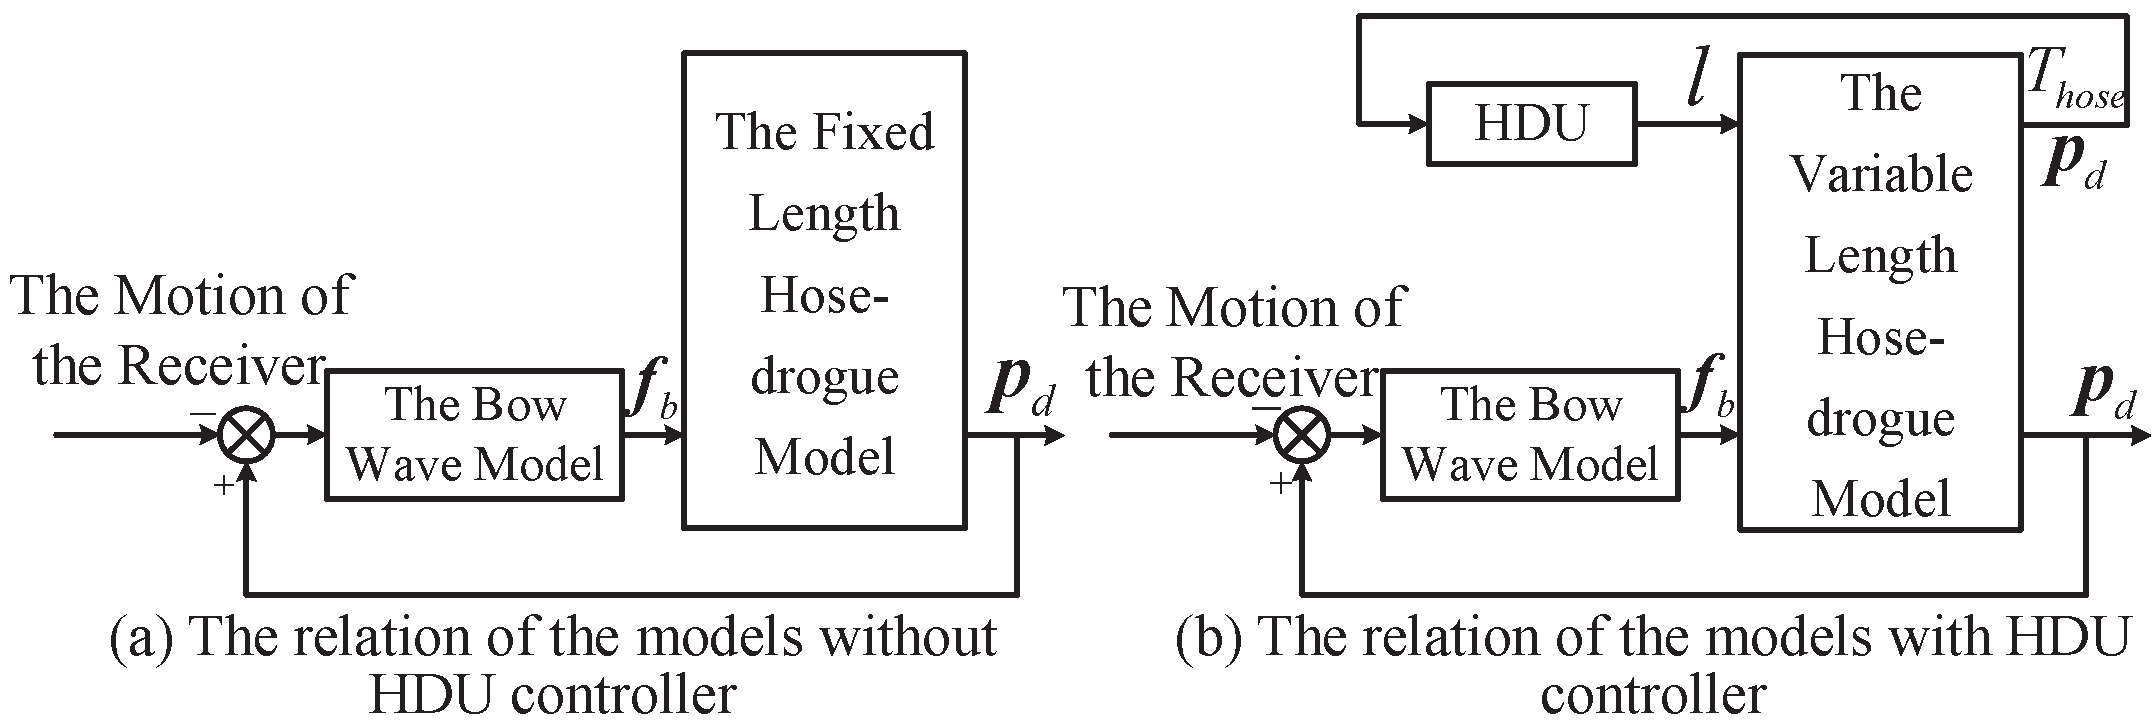
\includegraphics[width=0.80\textwidth]{Figures/Figs_Ch8/Fig06} 
		\par\end{centering}
	\caption{The relation between the models with and without HDU controller}
	\label{E_HDU1} 
\end{figure*}

The dynamic model of the HDU is determined by its controller, which will be elaborated on in the next section.

\subsection{HDU Controller and Qualitative Analysis of its Control Effect}

The controller of the HDU adjusts ${T_{{\rm{reel}}}}$ by using the state variables of the hose (such as ${T_{{\rm{hose}}}},{l_1}$ and ${\dot l_1}$) to indirectly control the length of the exposed hose, thereby regulating the hose tension and achieving equilibrium without causing hose whipping phenomenon. Fig. \ref{F_Sim_Schematic} illustrates the structural diagram of the link-connected hose-drogue model with the inclusion of the HDU.

(1)Two Types of Controllers for HDU

The first type of controller is the one proposed in Refs. \cite{vassberg_numerical_2004,ro_modeling_2010}.
\begin{equation}\label{eq4.122}
{T_{{\rm{reel}}}}\left( t \right) = {T_{{\rm{reel}}}}\left( 0 \right){\left[ {\frac{{{l_1}\left( t \right)}}{{{l_1}\left( 0 \right)}}} \right]^k},0 < {l_1}\left( t \right) \le {l_1}\left( 0 \right)
\end{equation}
That is, at $t = 0$, when the hose is just fully extended, ${T_{{\rm{reel}}}}\left( 0 \right)$ represents the tension at that moment, ${l_1}\left( 0 \right)$ is the length of the first link at that moment, and $k \in \mathbb{R}_{+}$ is the parameter of the controller. It can be observed from Eqs. (\ref{eq4.121}) and (\ref{eq4.122}) that when the hose is completely extended (which corresponds to the state at $t = 0$), the controller achieves equilibrium, and there is no change in the hose length.
\begin{figure}[th]
	\centering
	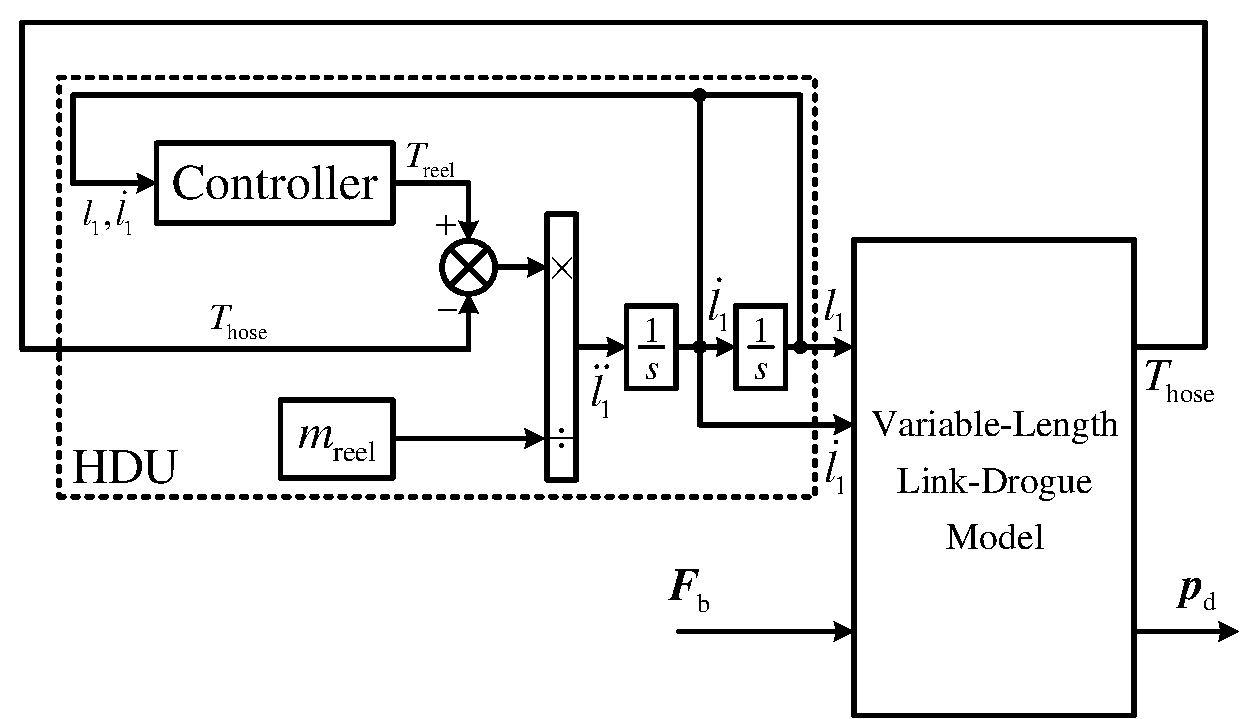
\includegraphics[width=0.7\textwidth]{Figures/Figs_Ch8/Fig07}
	\caption{Schematic of link-connected hose-drogue model with HDU}\label{F_Sim_Schematic}
\end{figure}
While the first type of controller does regulate the hose tension, its transient behavior is suboptimal. Therefore, based on the first type of controller, the second type of controller is proposed 
\begin{equation}\label{eq4.123}
{T_{{\rm{reel}}}}\left( t \right) = {T_{{\rm{reel}}}}\left( 0 \right){\left[ {\frac{{{l_1}\left( t \right)}}{{{l_1}\left( 0 \right)}}} \right]^k} + {k_d}{\dot l_1}\left( t \right),0 < {l_1}\left( t \right) \le {l_1}\left( 0 \right)
\end{equation}
where ${k_d} \in \mathbb{R}_{+}$. The second type of controller introduces a damping term ${k_d}{\dot l_1}\left( t \right)$, which can effectively improve the transient performance. Furthermore, since we can directly measure the linear velocity of the hose length change, or indirectly obtain the hose length change through the rotation speed of the drum, this controller is easy to implement.

Next, the HDU and the variable-length link-connected hose-drogue model will be used to simulate the control effects of the two types of controllers and analyze the effects of different $k$ values on each type of controller.

(2)Simulation and Qualitative Analysis of Two Types of Controllers

Firstly, establish the simulation model as shown in Fig. \ref{F_Sim_Schematic}. The basic settings of the simulation environment are outlined in Table II in Section 4.2. For the sake of convenience in simulation, some of the parameters listed in Table II in Section 4.2 have been modified in this chapter's simulations. Additionally, new simulation parameters related to the HDU have been added, as depicted in in Table III in Section 4.3.

Let the force ${\bm {f}_{\rm{b}}}$ experience a step change from ${\left[ {\begin{array}{*{20}{c}}
		0&0&0
		\end{array}} \right]^{\rm{T}}}$ to ${\left[ {\begin{array}{*{20}{c}}
		{75}&0&0
		\end{array}} \right]^{\rm{T}}}$ at 100 seconds. This is done to mimic the force difference in the ${o_{\rm{t}}}{x_{\rm{t}}}$ direction that contributed to the disparities between simulations and experiments in Section 4.3.4. For both the first type of controller and the second type of controller, select the controller parameters as $k = \left\{ {0.3,0.5,1,3} \right\}$, with ${k_d} = 500$ for the second type of controller.

The simulation results are presented in Fig. \ref{F_Effects}. Subfigures (a1)-(a4) depict the control effects of the first type of controller, while subfigures (b1)-(b4) illustrate the control effects of the second type of controller. Through comparison, the following conclusions can be qualitatively drawn:

1) Comparing subfigures (a1)-(a4) and (b1)-(b4) in Fig. \ref{F_Effects}, it can be observed that the first type of controller leads to pronounced oscillations with a longer settling time. In contrast, the second type of controller exhibits significant improvements in both tension adjustment and drogue position control, showing smoother transition dynamics than the first type of controller.

2) Comparing Fig. \ref{F_Effects} (a1) with Fig. \ref{F_Effects} (b1), it can be deduced that the parameter $k$ does not influence the steady-state value of the final hose tension.

3) Comparing Fig. \ref{F_Effects} (a1) with Fig. \ref{F_Effects} (b1), it can be observed that the parameter $k$ significantly affects the retraction length of the hose. When $k$ is smaller, the HDU needs to retract a longer length of the hose to achieve the same steady-state tension value. Conversely, if a minimal change in hose length is desired, a larger $k$ value can be chosen.

4) A larger value of $k$ brings about a noticeable negative effect, which makes the HDU-hose-drogue system unstable. This can be observed from Figs. \ref{F_Effects} (a1)-(a4), where the adjustment time of various quantities significantly increases with the increase in $k$. In fact, for the first type of controller with $k = 4$, the outputs of various quantities have already diverged. In contrast, comparing Figs. \ref{F_Effects} (b1)-(b4) reveals that the second type of controller shows significant improvement in addressing this phenomenon.

5) From Figs. \ref{F_Effects} (a3) and (a4) and Figs \ref{F_Effects} (b3) and (b4), it can be observed that the parameter $k$ indirectly influences the dynamics of the drogue in various directions by affecting the length of the hose. This characteristic will be further discussed in the subsequent sections of this chapter.
\begin{figure}[th]
	\centering
	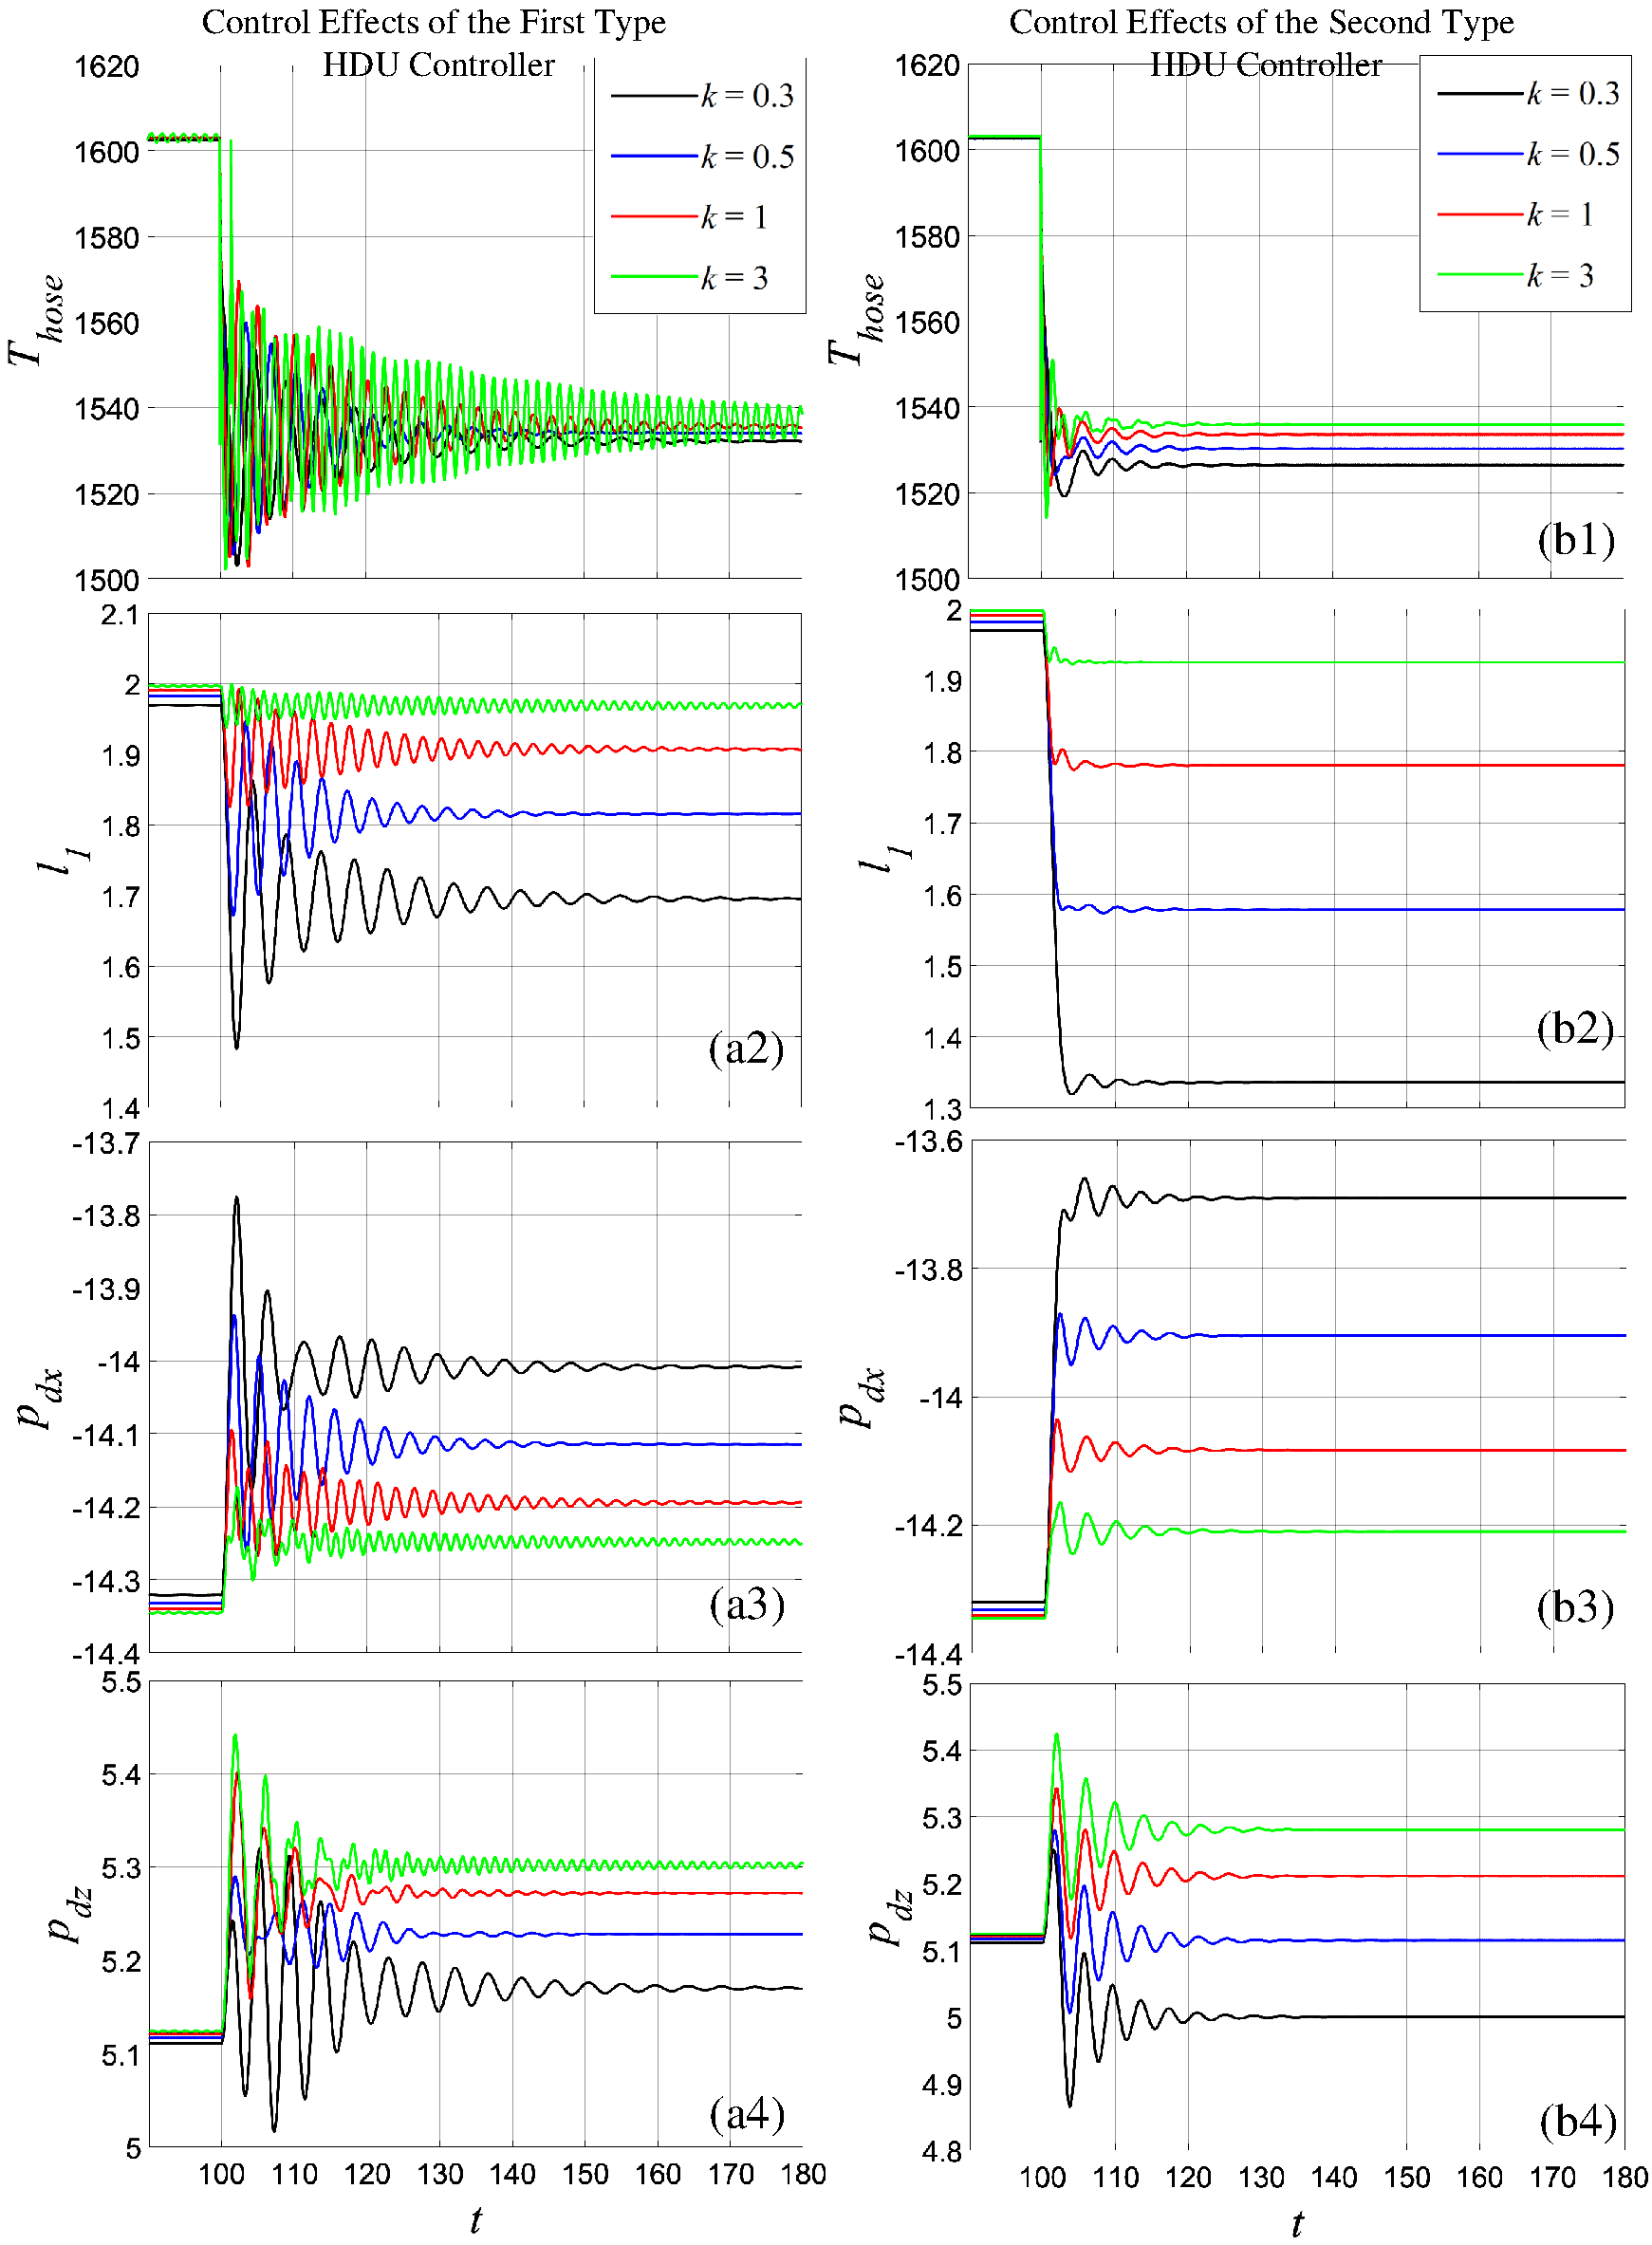
\includegraphics[width=0.7\textwidth]{Figures/Figs_Ch8/Fig08}
	\caption{Control Effects of Two Types of HDU Controllers}\label{F_Effects}
\end{figure} 

\section{Simplified Drogue Dynamic Model}
Regardless of whether the link-connected hose-drogue model includes the HDU, the model is too complex. As described in Section 4.2, to better simulate the dynamics of the hose, a significant number of links are required, with each link having multiple state variables such as ${\alpha _j},{\beta _j},{\dot \alpha _j},{\dot \beta _j},{l_j},{\dot l_j}$, etc. This complexity results in a high-order link-connected hose-drogue model. Additionally, the presence of nonlinear operations in model calculations further increases its complexity. However, when designing a docking controller, only the dynamics of the drogue are concerned with, and the dynamics of other links become redundant. Therefore, this section aims to simplify the link-connected hose-drogue model in order to obtain a model that solely expresses the dynamics of the drogue. This simplified model is referred to as the drogue dynamics model. It has a lower order and is suitable for controller design in subsequent chapters. Furthermore, it allows for quantitative analysis of the drogue's dynamics under different HDU models.

\subsection{Problem Description and Modeling Approach for Drogue Dynamic Model}

(1) Problem Description for Drogue Dynamic Model

In Section 4.3.1, the link-plexity results in a highorderconnected hose-drogue model was represented using Eq. (98). If taking the HDU model into account, with the drogue's forces as inputs and the drogue's position as output, the system can be expressed as follows 
\begin{equation}\label{E_Model}
\left\{ \begin{aligned}
&{{ {\dot {\bm{x}}}}_{{\rm{reel}}}} = { {{\bm{f}}}_{{\rm{reel}}}}\left( {{ {{\bm{x}}}_{{\rm{reel}}}},{ {{\bm{x}}}_{\rm{h}}}} \right)\\
&{{ {\dot {\bm{x}}}}_{\rm{h}}} = { {{\bm{f}}}_{{\rm{h0}}}}\left( {{ {{\bm{x}}}_{\rm{h}}},{ {{\bm{x}}}_{\rm{d}}}, {{\bm{v}}}_{{\rm{t/w}}}^{\rm{g}},h_{\rm{t}}^{\rm{g}}} \right)\\
&{{ {\dot {\bm{x}}}}_{\rm{d}}} = { {{\bm{f}}}_{{\rm{d0}}}}\left( {{ {{\bm{x}}}_{\rm{h}}},{ {{\bm{x}}}_{\rm{d}}}, {{\bm{v}}}_{{\rm{t/w}}}^{\rm{g}},h_{\rm{t}}^{\rm{g}},{ {{\bm{F}}}_{\rm{b}}}} \right)\\
&{ {{\bm{p}}}_{\rm{d}}} = { {{\bm{f}}}_y}\left( {{ {{\bm{x}}}_{\rm{h}}},{ {{\bm{x}}}_{\rm{d}}}} \right)
\end{aligned} \right.
\end{equation}
where ${ {{\bm{x}}}_{{\rm{reel}}}}$ represents the state variables of the HDU, and ${ {{\bm{f}}}_{{\rm{reel}}}}$ represents the function related to the dynamics of the HDU as described in Section 8.4. Under a constant tanker altitude ${h_0}$ and airspeed ${ \bm{v}_0}$, the model is simplified to 
\begin{equation}\label{E_SimplifiedModel}
\left\{ \begin{aligned}
&{{ {\dot {\bm{x}}}}_{{\rm{reel}}}} = { {{\bm{f}}}_{{\rm{reel}}}}\left( {{ {{\bm{x}}}_{{\rm{reel}}}},{ {{\bm{x}}}_{\rm{h}}}} \right)\\
&{{ {\dot {\bm{x}}}}_{\rm{h}}} = { {{\bm{f}}}_{\rm{h}}}\left( {{ {{\bm{x}}}_{{\rm{reel}}}},{ {{\bm{x}}}_{\rm{h}}},{ {{\bm{x}}}_{\rm{d}}}} \right)\\
&{{ {\dot {\bm{x}}}}_{\rm{d}}} = { {{\bm{f}}}_{\rm{d}}}\left( {{ {{\bm{x}}}_{\rm{h}}},{ {{\bm{x}}}_{\rm{d}}},{ {{\bm{F}}}_{\rm{b}}}} \right)\\
&{ {{\bm{p}}}_{\rm{d}}} = { {{\bm{f}}}_y}\left( {{ {{\bm{x}}}_{\rm{h}}},{ {{\bm{x}}}_{\rm{d}}}} \right)
\end{aligned} \right.
\end{equation}
where ${ {{\bm{f}}}_{\rm{h}}}\left( {{ {{\bm{x}}}_{\rm{h}}},{ {{\bm{x}}}_{\rm{d}}}} \right) \triangleq { {{\bm{f}}}_{{\rm{h0}}}}\left( {{ {{\bm{x}}}_{\rm{h}}},{ {{\bm{x}}}_{\rm{d}}},{ {{\bm{v}}}_0},{h_0}} \right),{ {{\bm{f}}}_{\rm{d}}}\left( {{ {{\bm{x}}}_{\rm{h}}},{ {{\bm{x}}}_{\rm{d}}},{ {{\bm{F}}}_{\rm{b}}}} \right) \triangleq { {{\bm{f}}}_{{\rm{d0}}}}\left( {{ {{\bm{x}}}_{\rm{h}}},{ {{\bm{x}}}_{\rm{d}}},{ {{\bm{v}}}_0},{h_0},{ {{\bm{F}}}_{\rm{b}}}} \right)$. Then, for each set of $\left( {{ {{\bm{v}}}_0},{h_0}} \right)$, and when the system (\ref{E_SimplifiedModel}) is subjected to zero input (i.e., ${ {{\bm{F}}}_{\rm{b}}} = {\bf{0}}$), the system will reach a steady-state position. Denote the state of the system at this time as the equilibrium state 
\begin{equation}\label{E_Equilibrium}
{ {{\bm{x}}}_{{\rm{reel}}}} =  {{\bm{x}}}_{{\rm{reel}}}^*,{ {{\bm{x}}}_{\rm{h}}} =  {{\bm{x}}}_{\rm{h}}^{\rm{*}},{ {{\bm{x}}}_{\rm{d}}} =  {{\bm{x}}}_{\rm{d}}^{\rm{*}}
\end{equation}
At this moment, the system satisfies the equation 
\begin{equation}\label{E_ModelEquilibrium}
\left\{ \begin{aligned}
&{\dot {\bm{x}}}_{{\rm{reel}}}^* = { {{\bm{f}}}_{{\rm{reel}}}}\left( { {{\bm{x}}}_{{\rm{reel}}}^*, {{\bm{x}}}_{\rm{h}}^{\rm{*}}} \right)\\
&{\dot {\bm{x}}}_{\rm{h}}^{\rm{*}} = { {{\bm{f}}}_{\rm{h}}}\left( { {{\bm{x}}}_{{\rm{reel}}}^*, {{\bm{x}}}_{\rm{h}}^{\rm{*}}, {{\bm{x}}}_{\rm{d}}^{\rm{*}}} \right)\\
&{\dot {\bm{x}}}_{\rm{d}}^{\rm{*}} = { {{\bm{f}}}_{\rm{d}}}\left( { {{\bm{x}}}_{\rm{h}}^{\rm{*}}, {{\bm{x}}}_{\rm{d}}^{\rm{*}},{\bf{0}}} \right)\\
&{{\bm{p}}}_{\rm{d}}^{\rm{*}} = { {{\bm{f}}}_y}\left( { {{\bm{x}}}_{\rm{h}}^{\rm{*}}, {{\bm{x}}}_{\rm{d}}^{\rm{*}}} \right)
\end{aligned} \right.
\end{equation}
Linearizing the system (\ref{E_SimplifiedModel}) at the equilibrium point (\ref{E_ModelEquilibrium}), we can obtain 
\begin{equation}\label{E_Linearizing}
\left\{ \begin{aligned}
\left[ {\begin{array}{*{20}{c}}
	{\Delta {{ {\dot {\bm{x}}}}_{{\rm{reel}}}}}\\
	{\Delta {{ {\dot {\bm{x}}}}_{\rm{h}}}}\\
	{\Delta {{ {\dot {\bm{x}}}}_{\rm{d}}}}
	\end{array}} \right] &= \underbrace {\left[ {\begin{array}{*{20}{c}}
		{{{\bf{A}}_{11}}}&{{{\bf{A}}_{12}}}&{\bf{0}}\\
		{{{\bf{A}}_{21}}}&{{{\bf{A}}_{22}}}&{{{\bf{A}}_{23}}}\\
		{\bf{0}}&{{{\bf{A}}_{32}}}&{{{\bf{A}}_{33}}}
		\end{array}} \right]}_{\bf{A}}\left[ {\begin{array}{*{20}{c}}
	{\Delta { {{\bm{x}}}_{{\rm{reel}}}}}\\
	{\Delta { {{\bm{x}}}_{\rm{h}}}}\\
	{\Delta { {{\bm{x}}}_{\rm{d}}}}
	\end{array}} \right] + \underbrace {\left[ {\begin{array}{*{20}{c}}
		{\bf{0}}\\
		{\bf{0}}\\
		{{{\bf{B}}_3}}
		\end{array}} \right]}_{\bf{B}}{\bm {F}_{\rm{b}}}{\rm{ + }}\left[ {\begin{array}{*{20}{l}}
	{o\left( {\Delta { {{\bm{x}}}_{{\rm{reel}}}},\Delta { {{\bm{x}}}_{\rm{h}}}} \right)}\\
	{o\left( {\Delta { {{\bm{x}}}_{{\rm{reel}}}},\Delta { {{\bm{x}}}_{\rm{h}}},\Delta { {{\bm{x}}}_{\rm{d}}}} \right)}\\
	{o\left( {\Delta { {{\bm{x}}}_{\rm{h}}},\Delta { {{\bm{x}}}_{\rm{d}}},{ {F}_{\rm{b}}}} \right)}
	\end{array}} \right]\\
\Delta { {{\bm{p}}}_{\rm{d}}} &= \underbrace {\left[ {\begin{array}{*{20}{c}}
		{\bf{0}}&{{{\bf{C}}_2}}&{{{\bf{C}}_3}}
		\end{array}} \right]}_{\bf{C}}\left[ {\begin{array}{*{20}{c}}
	{\Delta { {{\bm{x}}}_{{\rm{reel}}}}}\\
	{\Delta { {{\bm{x}}}_{\rm{h}}}}\\
	{\Delta { {{\bm{x}}}_{\rm{d}}}}
	\end{array}} \right] + o\left( {\Delta { {{\bm{x}}}_{\rm{h}}},\Delta { {{\bm{x}}}_{\rm{d}}}} \right)
\end{aligned} \right.
\end{equation}
where
\begin{equation}\label{E_LinearizingSub}
\begin{array}{*{20}{l}}
{{{\bf{A}}_{11}}{\rm{ = }}{{\left. {\frac{{\partial { {{\bm{f}}}_{{\rm{reel}}}}}}{{\partial { {{\bm{x}}}_{{\rm{reel}}}}}}} \right|}_{\scriptstyle{ {{\bm{x}}}_{{\rm{reel}}}} =  {{\bm{x}}}_{{\rm{reel}}}^*\hfill\atop
			\scriptstyle{ {{\bm{x}}}_{\rm{h}}} =  {{\bm{x}}}_{\rm{h}}^{\rm{*}}\hfill}},}&{{{\bf{A}}_{12}}{\rm{ = }}{{\left. {\frac{{\partial { {{\bm{f}}}_{{\rm{reel}}}}}}{{\partial { {{\bm{x}}}_{\rm{h}}}}}} \right|}_{\scriptstyle{ {{\bm{x}}}_{{\rm{reel}}}} =  {{\bm{x}}}_{{\rm{reel}}}^*\hfill\atop
			\scriptstyle{ {{\bm{x}}}_{\rm{h}}} =  {{\bm{x}}}_{\rm{h}}^{\rm{*}}\hfill}},}&{{{\bf{A}}_{21}}{\rm{ = }}{{\left. {\frac{{\partial { {{\bm{f}}}_{\rm{h}}}}}{{\partial { {{\bm{x}}}_{{\rm{reel}}}}}}} \right|}_{\scriptstyle{ {{\bm{x}}}_{{\rm{reel}}}} =  {{\bm{x}}}_{{\rm{reel}}}^*\hfill\atop
			{\scriptstyle{ {{\bm{x}}}_{\rm{h}}} =  {{\bm{x}}}_{\rm{h}}^{\rm{*}}\hfill\atop
				\scriptstyle{ {{\bm{x}}}_{\rm{d}}} =  {{\bm{x}}}_{\rm{d}}^{\rm{*}}\hfill}}},}&{{{\bf{A}}_{22}}{\rm{ = }}{{\left. {\frac{{\partial { {{\bm{f}}}_{\rm{h}}}}}{{\partial { {{\bm{x}}}_{\rm{h}}}}}} \right|}_{\scriptstyle{ {{\bm{x}}}_{{\rm{reel}}}} =  {{\bm{x}}}_{{\rm{reel}}}^*\hfill\atop
			{\scriptstyle{ {{\bm{x}}}_{\rm{h}}} =  {{\bm{x}}}_{\rm{h}}^{\rm{*}}\hfill\atop
				\scriptstyle{ {{\bm{x}}}_{\rm{d}}} =  {{\bm{x}}}_{\rm{d}}^{\rm{*}}\hfill}}},}\\
{{{\bf{A}}_{23}}{\rm{ = }}{{\left. {\frac{{\partial { {f}_{\rm{h}}}}}{{\partial { {{\bm{x}}}_{\rm{d}}}}}} \right|}_{\scriptstyle{ {{\bm{x}}}_{{\rm{reel}}}} =  {{\bm{x}}}_{{\rm{reel}}}^*\hfill\atop
			{\scriptstyle{ {{\bm{x}}}_{\rm{h}}} =  {{\bm{x}}}_{\rm{h}}^{\rm{*}}\hfill\atop
				\scriptstyle{ {{\bm{x}}}_{\rm{d}}} =  {{\bm{x}}}_{\rm{d}}^{\rm{*}}\hfill}}},}&{{{\bf{A}}_{32}}{\rm{ = }}{{\left. {\frac{{\partial { {{\bm{f}}}_{\rm{d}}}}}{{\partial { {{\bm{x}}}_{\rm{h}}}}}} \right|}_{\scriptstyle{ {{\bm{x}}}_{\rm{h}}} =  {{\bm{x}}}_{\rm{h}}^{\rm{*}}\hfill\atop
			{\scriptstyle{ {{\bm{x}}}_{\rm{d}}} =  {{\bm{x}}}_{\rm{d}}^{\rm{*}}\hfill\atop
				\scriptstyle{ {F}_{\rm{b}}} = 0\hfill}}},}&{{{\bf{A}}_{33}}{\rm{ = }}{{\left. {\frac{{\partial { {{\bm{f}}}_{\rm{d}}}}}{{\partial { {{\bm{x}}}_{\rm{d}}}}}} \right|}_{\scriptstyle{ {{\bm{x}}}_{\rm{h}}} =  {{\bm{x}}}_{\rm{h}}^{\rm{*}}\hfill\atop
			{\scriptstyle{ {{\bm{x}}}_{\rm{d}}} =  {{\bm{x}}}_{\rm{d}}^{\rm{*}}\hfill\atop
				\scriptstyle{ {F}_{\rm{b}}} = 0\hfill}}},}&{{{\bf{B}}_3}{\rm{ = }}{{\left. {\frac{{\partial { {{\bm{f}}}_{\rm{d}}}}}{{\partial { {{\bm{f}}}_{\rm{b}}}}}} \right|}_{\scriptstyle{ {{\bm{x}}}_{\rm{h}}} =  {{\bm{x}}}_{\rm{h}}^{\rm{*}}\hfill\atop
			{\scriptstyle{ {{\bm{x}}}_{\rm{d}}} =  {{\bm{x}}}_{\rm{d}}^{\rm{*}}\hfill\atop
				\scriptstyle{ {F}_{\rm{b}}} = 0\hfill}}},}\\
{{{\bf{C}}_2}{\rm{ = }}{{\left. {\frac{{\partial { {{\bm{f}}}_y}}}{{\partial { {{\bm{x}}}_{\rm{h}}}}}} \right|}_{\scriptstyle{ {{\bm{x}}}_{\rm{h}}} =  {{\bm{x}}}_{\rm{h}}^{\rm{*}}\hfill\atop
			\scriptstyle{ {{\bm{x}}}_{\rm{d}}} =  {{\bm{x}}}_{\rm{d}}^{\rm{*}}\hfill}},}&{{{\bf{C}}_3}{\rm{ = }}{{\left. {\frac{{\partial { {{\bm{f}}}_y}}}{{\partial { {{\bm{x}}}_{\rm{d}}}}}} \right|}_{\scriptstyle{ {{\bm{x}}}_{\rm{h}}} =  {{\bm{x}}}_{\rm{h}}^{\rm{*}}\hfill\atop
			\scriptstyle{ {{\bm{x}}}_{\rm{d}}} =  {{\bm{x}}}_{\rm{d}}^{\rm{*}}\hfill}}}&{}&{}
\end{array}
\end{equation}
and $\Delta { {{\bm{x}}}_{{\rm{reel}}}} = { {{\bm{x}}}_{{\rm{reel}}}} -  {{\bm{x}}}_{{\rm{reel}}}^*,\Delta { {{\bm{x}}}_{\rm{h}}} = { {{\bm{x}}}_{\rm{h}}} -  {{\bm{x}}}_{\rm{h}}^*,\Delta { {{\bm{x}}}_{\rm{d}}} = { {{\bm{x}}}_{\rm{d}}} -  {{\bm{x}}}_{\rm{d}}^*,\Delta { {{\bm{p}}}_{\rm{d}}} = { {{\bm{p}}}_{\rm{d}}} -  {{\bm{p}}}_{\rm{d}}^{\rm{*}}$, according to the drogue equilibrium coordinate system, it can be observed that $\Delta { {{\bm{p}}}_{\rm{d}}} =  {{\bm{p}}}_{\rm{d}}^{\rm{e}}$, and $o(\cdot)$ represents higher-order infinitesimal terms in the linearization. Since the changes in the state of the hose and the drogue are relatively small during the docking process, i.e., $\Delta { {{\bm{x}}}_{{\rm{reel}}}},\Delta { {{\bm{x}}}_{\rm{h}}}$ and $\Delta { {{\bm{x}}}_{\rm{d}}}$ are infinitesimal terms that can be neglected. Additionally, if the subsequent model simplification can be validated through the process described in section 8.3.4, it would also indicate the reasonableness of omitting infinitesimal terms here. After neglecting infinitesimal terms, the system (\ref{E_Linearizing}) becomes a linear system. Subsequently, through Laplace transformation, the transfer function of this linear system can be expressed as 
\begin{equation}\label{E_Transfer}
{{\bm{p}}}_{\rm{d}}^{\rm{e}}\left( s \right) = \underbrace {{\bf{C}}{{\left( {s{\bf{I}} - {\bf{A}}} \right)}^{ - 1}}{\bf{B}}}_{{{\bf{G}}_{\rm{d}}}\left( s \right)}{ {{\bm{F}}}_{\rm{b}}}\left( s \right)
\end{equation}
This equation is commonly referred to as the drogue dynamic model.

(2) Modeling Approach for Drogue Dynamic Model

The model (\ref{E_Transfer}) includes ${{\bf{G}}_{\rm{d}}}\left( s \right)$, which represents the drogue's dynamics. Next, system identification methods will be used to obtain ${{\bf{G}}_{\rm{d}}}\left( s \right)$, and the following steps outline this process:

1) Utilize axial force to infer the coupling relationships among different channels, and then obtain the basic form of ${{\bf{G}}_{\rm{d}}}\left( s \right)$.

2) Employ Generalized Binary Noise (GBN) as an input to excite the system and identify system parameters.

3) Validate the identified results using a Chirp Signal.

In Sections 8.3.2-8.3.4, we will combine an example of a fixed-length link-connected model to explain the above process. The object to be identified in this example is the same as the one in Section 4.2.5. The obtained drogue dynamic model can be analyzed and compared with the later derived link-connected hose-drogue model with HDU.

\subsection{Speculation on the Form of ${{\bf{G}}_{\rm{d}}}\left( s \right)$}

Five simulations are conducted, each applying an axial force in a different direction to ${\bm{F}_{\rm{b}}}$. The forces were as follows  ${\bm{F}_{{\rm{b}}x{\rm{ + }}}} = {\left[ {\begin{array}{*{20}{c}}
		{50}&0&0
		\end{array}} \right]^{\rm{T}}}$, ${\bm{F}_{{\rm{b}}y{\rm{ + }}}} = {\left[ {\begin{array}{*{20}{c}}
		0&{50}&0
		\end{array}} \right]^{\rm{T}}}$, ${\bm{F}_{{\rm{b}}y - }} = {\left[ {\begin{array}{*{20}{c}}
		0&{ - 50}&0
		\end{array}} \right]^{\rm{T}}}$, ${\bm{F}_{{\rm{b}}z{\rm{ + }}}} = {\left[ {\begin{array}{*{20}{c}}
		0&0&{50}
		\end{array}} \right]^{\rm{T}}}$, ${\bm{F}_{{\rm{b}}z{\rm{ + }}}} = {\left[ {\begin{array}{*{20}{c}}
		0&0&{ - 50}
		\end{array}} \right]^{\rm{T}}}$. The reason for not using forces in the ${\bm{F}_{{\rm{b}}x - }}$ direction for simulation is that, under normal circumstances, the receiver does not generate disturbances in the negative direction against the drogue. The choice of an amplitude of $50 N$ is because the maximum bow wave effect during the docking process is around $100 N$, and $50 N$ serves as a representative intermediate value for the bow wave effect. The results of these five simulations are presented in Table \ref{T_SimEnvironment}. In the table, $(\cdot)_\text{max}$ represents the maximum drift position of the drogue in the current simulation, while $(\cdot)_\text{final}$ represents the final drift position of the drogue in the current simulation.

% Table generated by Excel2LaTeX from sheet 'Sheet1'
\begin{table}[htbp]
	\centering
	\caption{Parameters Used in HDU Simulation}
	\begin{tabular}{|l|c|c|}
		\hline Parameters    & Values & Units \\ \hline
		Number of Link Segments $N$  & $10$    & - \\ \hline
		Full length of the hose, $L_{h}$  & 15  & m \\ \hline 
		Initial Length of the First Link ${l_1}\left( 0 \right)$ & $2$     & $m$ \\ \hline
		Lengths of the Remaining Links ${l_j}\left( 0 \right),j = 2,3, \ldots ,N$ & $13/9$  & $m$ \\ \hline
		The Mass of the Reel ${m_{{\rm{reel}}}}$& $68$    & $kg$ \\ \hline
		Initial Tension of the Reel  & 1610  & $N$ \\ \hline
	\end{tabular}%
	\label{T_SimEnvironment}%
\end{table}%

According to Table \ref{T_SimEnvironment}, the following conclusions can be drawn: 1) The $x$ and $z$ channels are coupled. 2) It can be assumed that the $y$ channel is decoupled from $x$ and $z$ channels, as the effects of ${\bm{F}_{{\rm{b}}y{\rm{ + }}}}$ and ${\bm{F}_{{\rm{b}}y - }}$ on ${x_{{d /t}}}$ and ${z_{{d /t}}}$ are much smaller than the forces in other directions. Therefore, the basic form of ${{\bf{G}}_{\rm{d}}}\left( s \right)$ can be obtained as follows 
\begin{equation}\label{E_BasicForm}
{{\bf{G}}_{\rm{d}}}\left( s \right) = \left[ {\begin{array}{*{20}{c}}
	{{G_{xx}}\left( s \right)}&0&{{G_{xz}}\left( s \right)}\\
	0&{{G_{yy}}\left( s \right)}&0\\
	{{G_{zx}}\left( s \right)}&0&{{G_{zz}}\left( s \right)}
	\end{array}} \right]
\end{equation}

Additionally, in Section 4.2.5, it has been mentioned that the inherent dynamics of the drogue are of second order. Therefore, it can be inferred that the elements within ${{\bf{G}}_{\rm{d}}}\left( s \right)$ are also of second order.

\subsection{System identification of the link-connected hose-drogue model}

Using a GBN (Generalized Binary Noise) signal with an amplitude of $50 N$ to excite the system, as shown in Fig. \ref{F_GBN}, the parameters within ${{\bf{G}}_{\rm{d}}}\left( s \right)$ are identified using the Output-Error (OE) model \cite{ljung_system_1998}. The results can be obtained as follows 
\begin{equation}\label{E_IdentifyResult}
\left\{ \begin{array}{c}
{G_{xx}}\left( s \right){\rm{ = }}\frac{{{\rm{0}}{\rm{.002185}}}}{{{s^2} + {\rm{0}}{\rm{.3071}}s + {\rm{2}}{\rm{.682}}}}\\
{G_{xz}}\left( s \right){\rm{ = }}\frac{{{\rm{0}}{\rm{.006169}}}}{{{s^2} + {\rm{0}}{\rm{.3013}}s + {\rm{2}}{\rm{.689}}}}\\
{G_{yy}}\left( s \right){\rm{ = }}\frac{{{\rm{0}}{\rm{.01712}}}}{{{s^2} + {\rm{0}}{\rm{.2422}}s + {\rm{2}}{\rm{.081}}}}\\
{G_{zx}}\left( s \right){\rm{ = }}\frac{{{\rm{0}}{\rm{.005824}}}}{{{s^2} + {\rm{0}}{\rm{.3223}}s + {\rm{2}}{\rm{.687}}}}\\
{G_{zz}}\left( s \right){\rm{ = }}\frac{{{\rm{0}}{\rm{.01782}}}}{{{s^2} + {\rm{0}}{\rm{.3391}}s + {\rm{2}}{\rm{.687}}}}
\end{array} \right..
\end{equation}

\subsection{Frequency sweep verification}

A frequency sweep signal is simultaneously applied to both the link-connected hose-drogue model (Equation \ref{E_SimplifiedModel}) and the drogue dynamics model (Equation \ref{E_Transfer}), as shown in Fig. \ref{F_Verification_Framework}. By comparing the output results of the two systems, the simulation results are presented in Fig. \ref{F_System_Identification}. The curves in Fig. \ref{F_System_Identification}(b) are obtained by subtracting the two dashed lines from Fig. \ref{F_System_Identification}(a). The frequency sweep signal is a signal with a fixed amplitude and a frequency that uniformly increases from ${\zeta _0}$ to ${\zeta _T}$ over the interval $\left[ {0,T} \right]$, and its mathematical expression is 
\begin{equation}\label{E_Frequency}
c\left( t \right) = {{\rm{K}}_c}\sin \left[ {2\pi \left( {{\zeta _0} + \frac{{{\zeta _T} - {\zeta _0}}}{T}t} \right)t} \right]
\end{equation}
where ${{\rm{K}}_c} = 50,{\zeta _0} = 0.05Hz,{\zeta _T} = 0.5Hz$ and $T = 200s$.
\begin{figure}[th]
	\centering
	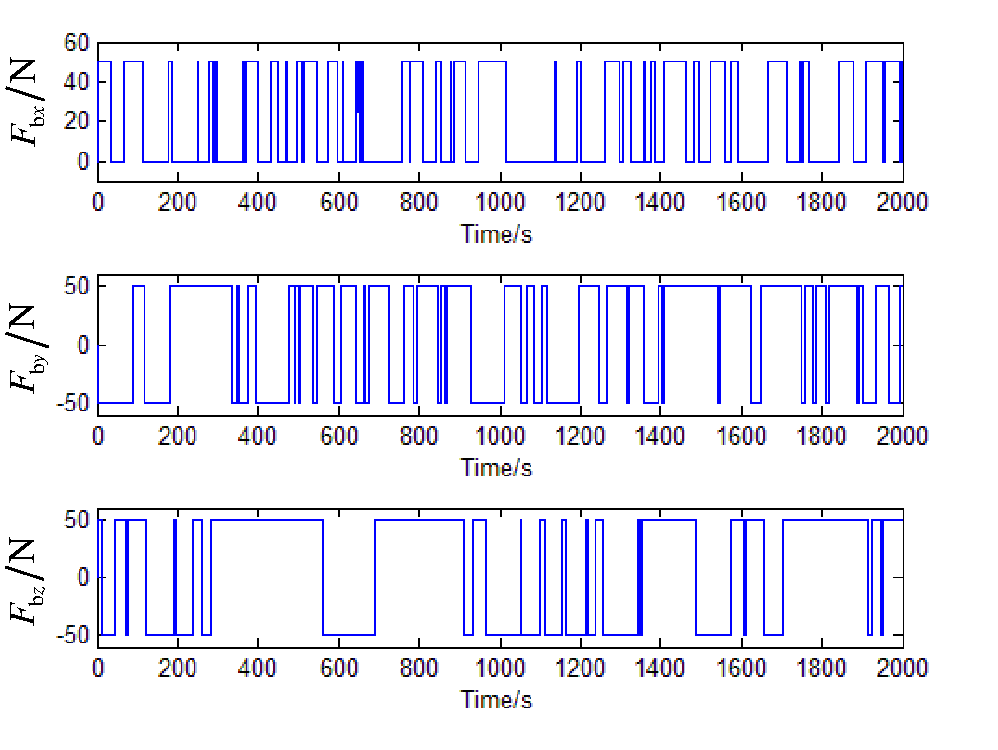
\includegraphics[width=0.7\textwidth]{Figures/Figs_Ch8/Fig09}
	\caption{GBN Signal Used to Excite the System}\label{F_GBN}
\end{figure} 
\begin{figure}[th]
	\centering
	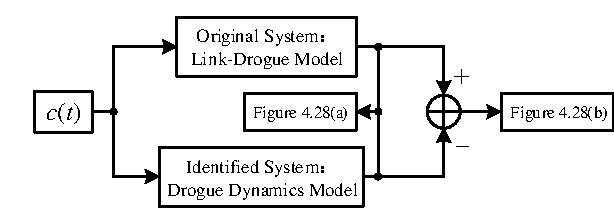
\includegraphics[width=0.7\textwidth]{Figures/Figs_Ch8/Fig10}
	\caption{Verification Simulation Framework for Identification Results}\label{F_Verification_Framework}
\end{figure} 
\begin{figure}[th]
	\centering
	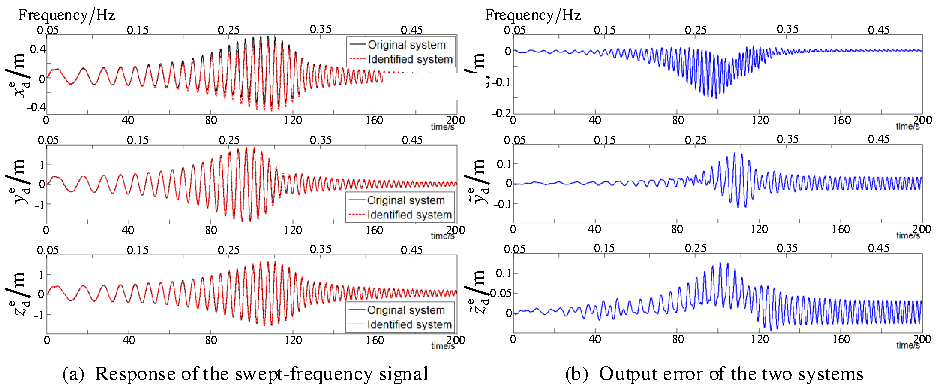
\includegraphics[width=0.7\textwidth]{Figures/Figs_Ch8/Fig11}
	\caption{Effectiveness of System Identification}\label{F_System_Identification}
\end{figure} 
From Fig. \ref{F_System_Identification} (b), it can be observed that the system's tracking error is minimal in the low-frequency range below 0.2 Hz, increases in the mid-frequency range between 0.2 Hz and 0.35 Hz, and remains relatively small in the high-frequency range above 0.35 Hz. The outputs $y_{\rm{d}}^{\rm{e}}$ and $z_{\rm{d}}^{\rm{e}}$ from both models are very close to each other, while the performance of $x_{\rm{d}}^{\rm{e}}$ is relatively poorer. This is mainly due to the higher nonlinearity exhibited by the link-connected hose-drogue model when subjected to ${\bm{F}_{{\rm{b}}x - }}$, which occurs rarely in actual docking scenarios. Therefore, the identified drogue dynamics model effectively captures the drogue dynamics of the link-connected hose-drogue model.

It should be noted that the above model was derived under the assumption of no crosswind or minimal crosswind. In the presence of a crosswind, the $y$-axis becomes coupled with the other axes, meaning that all elements within Eq. (\ref{E_BasicForm}) would be non-zero. However, the drogue dynamics model can still be obtained using the identification method described above. Since the refueling process allows for adjustments in the direction of the aircraft's velocity to minimize the impact of crosswind disturbances, this chapter primarily focuses on the model under the assumption of no crosswind.

\subsection{Dynamic Model of Drogue with HDU and Quantitative Analysis}

Using the system identification steps described in Sections 8.3.2-8.3.4, the simplified drogue dynamics model for the link-connected hose-drogue system with HDU was obtained. The identification results are presented in Table \ref{T_DriftPosition}. The controller choices are as shown in Section 4.3.3: for the first type of HDU controller (\ref{eq4.122}), the parameter is set as $k = 0.5$, and for the second type of HDU controller (\ref{eq4.123}), the parameters are chosen as $k = 0.5$ and ${k_d} = 500$. In the table, the fitness metric is used to represent the identification performance, defined as $1 - {{\left\| {\bm{y} - \bm{\hat y}} \right\|} /{\left\| {\bm{y} - \bm{\bar y}} \right\|}}$, where $\bm{y},\bm{\hat y}$ and $\bm{\bar y}$ represent the output of the original model, the the output of the identification model, and the mean of the output of the original model, respectively.

% Table generated by Excel2LaTeX from sheet 'Sheet1'
\begin{table}[htbp]
	\centering
	\caption{Drift positions of the drogue under the influence of Fb in different directions}
	\begin{tabular}{|c|c|c|c|c|c|}
		\hline \diagbox{${\bm{p}_{{d /t}}}$}{${\bm{F}_{\rm{b}}}$}& ${\bm{F}_{{\rm{b}}x{\rm{ + }}}}$ & ${\bm{F}_{{\rm{b}}y{\rm{ + }}}}$ &   ${\bm{F}_{{\rm{b}}y - }}$    &   ${\bm{F}_{{\rm{b}}z{\rm{ + }}}}$    & ${\bm{F}_{{\rm{b}}z - }}$ \\\hline
		${\left( {{x_{{d /t}}}} \right)_{\max }}$& 0.07  & 0.015 & 0.015 & 0.204 & 0.177 \\\hline
		${\left( {{x_{{d/t}}}} \right)_{{\rm{final}}}}$& 0.04  & 0.005 & 0.005 & 0.109 & 0.105 \\\hline
		${\left( {{y_{{d/t}}}} \right)_{\max }}$& 0     & 0.724 & -0.724 & 0     & 0 \\\hline
		${\left( {{y_{{d / t}}}} \right)_{{\rm{final}}}}$& 0     & 0.41  & -0.41 & 0     & 0 \\\hline
		${\left( {{z_{{d/ t}}}} \right)_{\max }}$& 0.199 & -0.012 & -0.012 & 0.56  & -0.588 \\\hline
		${\left( {{z_{{d / t}}}} \right)_{{\rm{final}}}}$& 0.115 & -0.004 & -0.004 & 0.324 & -0.447 \\\hline
	\end{tabular}%
	\label{T_DriftPosition}%
\end{table}%

Unlike the drogue dynamics without considering HDU (Eq. (\ref{E_Transfer})), the identification in Table \ref{T_DriftPosition} utilizes a fourth-order model. The reason behind this choice is that the drogue dynamics without HDU are second-order, while the HDU itself introduces an additional second-order dynamics. Hence, a fourth-order model is employed to identify the link-connected hose-drogue system with HDU. Moreover, judging from the fitness values in the identification results, the fourth-order model also performs better than the second-order model. From Table \ref{T_DriftPosition}, the following conclusions regarding the drogue dynamics can be drawn:

1) The transition process under the control of the second-class controller exhibits significantly better performance compared with the first-class controller. This is due to the fact that, in comparison to the first-class controller, the poles of the drogue dynamic model under the second-class controller are far from the imaginary axis.

2) From the fitness values in Table \ref{T_DriftPosition}, it is evident that the identification results of the drogue dynamics under the control of the first-class controller are inferior to those under the second-class controller. This is due to the higher level of nonlinearity exhibited by the drogue dynamics under the first-class controller, which is also evident from Figs. \ref{F_Effects} (a3) and (a4). Therefore, if a more accurate drogue dynamic model is desired, employing the second-class controller for HDU control is more appropriate.

% Table generated by Excel2LaTeX from sheet 'Sheet1'
\begin{table}[htbp]
	\centering
	\caption{Drogue Dynamic Model Considering HDU (Controller Parameter $k=0.5$)}
	\begin{tabular}{|c|r|r|r|}
		\hline \diagbox{Controller}{Results} & \multicolumn{2}{c|}{Transfer function} & \multicolumn{1}{l|}{Fitness} \\ \hline
		\multirow{5}[0]{*}{First-Class HDU Controller} &   ${G_{xx}}\left( s \right)$    &    $\frac{{0.012{s^2} + 0.012s + 0.052}}{{{s^4} + 2.15{s^3} + 9.17{s^2} + 7.54s + {\rm{18}}{\rm{.21}}}}$   &$89.4\% $  \\ \cline{2-4}
		&    ${G_{xz}}\left( s \right)$   &   $\frac{{0.0010{s^2} + 0.0057s + 0.046}}{{{s^4} + 13.49{s^3} + 19.29{s^2} + 35.69s + {\rm{29}}{\rm{.50}}}}$    &$70.9\% $  \\ \cline{2-4}
		&    ${G_{yy}}\left( s \right)$   &   $\frac{{0.026{s^2} + 0.0034s + 0.42}}{{{s^4} + 0.39{s^3} + 24.02{s^2} + 5.76s + {\rm{49}}{\rm{.66}}}}$    &  $99.5\% $\\ \cline{2-4}
		&    ${G_{zx}}\left( s \right)$   &   $\frac{{0.0026{s^2} + 0.010s + 0.032}}{{{s^4} + 1.76{s^3} + 11.03{s^2} + 7.04s + {\rm{20}}{\rm{.01}}}}$    & $85.1\% $ \\ \cline{2-4}
		&    ${G_{zz}}\left( s \right)$   &   $\frac{{0.027{s^2} + 0.0011s + 0.38}}{{{s^4} + 0.56{s^3} + 24.22{s^2} + 7.06s + {\rm{53}}{\rm{.95}}}}$    & $94.5\% $ \\ \hline
		\multirow{5}[0]{*}{Second-Class HDU Controller} &   ${G_{xx}}\left( s \right)$   &   $\frac{{0.0090{s^2} + 0.011s + 0.021}}{{{s^4} + 4.01{s^3} + 6.61{s^2} + 10.48s + {\rm{7}}{\rm{.38}}}}$    & $98.3\% $ \\ \cline{2-4}
		&    ${G_{xz}}\left( s \right)$   &    $\frac{{0.0048{s^2} + 0.019s + 0.0085}}{{{s^4} + 3.29{s^3} + 5.77{s^2} + 8.44s + {\rm{5}}{\rm{.80}}}}$   & $98.5\% $ \\ \cline{2-4}
		&    ${G_{yy}}\left( s \right)$   &   $\frac{{0.026{s^2} + 0.0033s + 0.42}}{{{s^4} + 0.40{s^3} + 24.01{s^2} + 5.75s + {\rm{49}}{\rm{.62}}}}$    & $99.6\% $ \\ \cline{2-4}
		&    ${G_{zx}}\left( s \right)$   &   $\frac{{0.0051{s^2} + 0.0091s + 0.0051}}{{{s^4} + 1.96{s^3} + 4.32{s^2} + 4.71s + {\rm{3}}{\rm{.14}}}}$    & $93.2\% $ \\ \cline{2-4}
		&    ${G_{zz}}\left( s \right)$   &    $\frac{{0.027{s^2} + 0.0046s + 0.39}}{{{s^4} + 0.61{s^3} + 24.05{s^2} + 7.71s + {\rm{55}}{\rm{.76}}}}$   & $89.4\% $ \\ \hline
	\end{tabular}%
	\label{T_Fitness}%
\end{table}%

3) By comparing Table \ref{T_DriftPosition} with the transfer function in Eq. (\ref{E_Transfer}), it can be observed that the presence or absence of HDU significantly affects the drogue dynamics. Next, the impact of HDU on the drogue dynamics will be further analyzed by comparing their Direct Current Gain (DC Gain) of the transfer functions \cite{franklin_feedback_2015}. Taking the coefficients of the two classes of controllers as $k = \left\{ {0.3,0.5,1,3} \right\}$, the results are shown in Table \ref{T_Fitness}.

Based on Table \ref{T_Fitness}, the following conclusions can be drawn regarding the drogue dynamics.

1) The gains of the drogue dynamics models under both types of controllers are similar. In other words, the second type of controller only affects the transient behavior, while the steady-state values of both types are the same.

2) The primary factor influencing the DC gain is the controller coefficient $k$. The smaller the value of $k$, the more pronounced the impact, especially on ${G_{xx}}\left( s \right)$ and ${G_{zx}}\left( s \right)$. In this case, the decoupling between the $x$-channel and  $z$-channel is better, indicated by the fact that the gains of ${G_{zx}}\left( s \right)$ and ${G_{xz}}\left( s \right)$ are much smaller than those of ${G_{xx}}\left( s \right)$ and ${G_{zz}}\left( s \right)$. Conversely, as $k$ increases, coupling becomes more pronounced. For instance, when $k = 3$, the DC gain of the drogue dynamics model with HDU is already approaching that of the model without HDU.

3) The impact of HDU on the DC gain of the y-axis is not significant.

In summary, when designing HDU controllers with the aim of mitigating the hose whipping phenomenon, a larger value of $k$ should be selected. This choice would require fewer adjustments to achieve regulation and speed up the adjustment process. On the other hand, if the intention is to decouple the dynamics of the drogue, facilitating controller design, a smaller value of $k$ should be chosen. Therefore, the selection of $k$ should balance between these two aspects.

% Table generated by Excel2LaTeX from sheet 'Sheet1'
\begin{table}[htbp]
	\centering
	\caption{DC gain of drogue dynamic model model with or without HDU (order of magnitude is $10^{-4}$)}
	\begin{tabular}{|c|c|c|c|c|c|c|}
		\hline \multirow{2}[0]{*}{\diagbox{Transfer function}{Drogue model type}} & \multicolumn{5}{c|}{Considering HDU}             & \multirow{2}[0]{*}{Without considering HDU} \\ \cline{2-6}
		& HDU Controller & $k = 0.3$     & $k = 0.5$     & $k = 1$     & $k = 3$     &  \\ \hline
		\multirow{2}[0]{*}{ ${G_{xx}}\left( s \right)$}     & First-Class   & 41.6  & 28.69 & 18.96 & 12.59 &  \multirow{2}[0]{*}{8.15} \\ \cline{2-6}
		& Second-Class   & 42.04 & 28.98 & 19.15 & 12.64 &  \\ \hline
		\multirow{2}[0]{*}{ ${G_{xz}}\left( s \right)$}     & First-Class   & 8.08  & 14.48 & 20.07 & 23.56 & \multirow{2}[0]{*}{22.94} \\ \cline{2-6}
		& Second-Class   & 7.42  & 14.56 & 19.93 & 23.52 &  \\ \hline
		\multirow{2}[0]{*}{ ${G_{yy}}\left( s \right)$}     & First-Class   & 84.65 & 84.58 & 84.72 & 84.75 & \multirow{2}[0]{*}{82.29} \\ \cline{2-6}
		& Second-Class   & 84.65 & 84.68 & 84.73 & 84.75 &  \\ \hline
		\multirow{2}[0]{*}{ ${G_{zx}}\left( s \right)$}     & First-Class   & 11.81 & 15.98 & 19.78 & 21.77 & \multirow{2}[0]{*}{8.15} \\ \cline{2-6}
		& Second-Class   & 11.48 & 16.31 & 19.54 & 21.78 &  \\ \hline
		\multirow{2}[0]{*}{ ${G_{zz}}\left( s \right)$}     & First-Class   & 72.42 & 69.99 & 68.22 & 67.13 & \multirow{2}[0]{*}{66.32} \\ \cline{2-6}
		& Second-Class   & 72.02 & 69.76 & 68.2  & 67.08 &  \\ \hline
	\end{tabular}%
	\label{tab4.7}%
\end{table}%

If establishing a simulation environment similar to the one in Section 4.3.4 and replaceing the link-connected hose-drogue model with the drogue dynamic model with HDU (as shown in Table \ref{T_DriftPosition}), simulation results as depicted in Fig. \ref{F_Comparison} can be obtained. To visually display the differences in drogue dynamics with and without HDU during the docking process, as well as the differences in drogue dynamics under different controllers, a video have also been recorded. Readers can refer to Ref. \cite{noauthor_drogue_nodate-1} for the video, and a screenshot from the video is shown in Fig. \ref{F_Sim_Subsidence}. In the screenshot, View 1 represents the pilot's perspective, and View 2 provides a lateral view. The HDU used in the screenshot employs the first type of controller, which is common in current HDU designs. This choice accurately reflects the flight conditions in the experiment. To compare with the results from Ref. \cite{dibley_autonomous_2007}, the units for position are given in feet.
\begin{figure}[th]
	\centering
	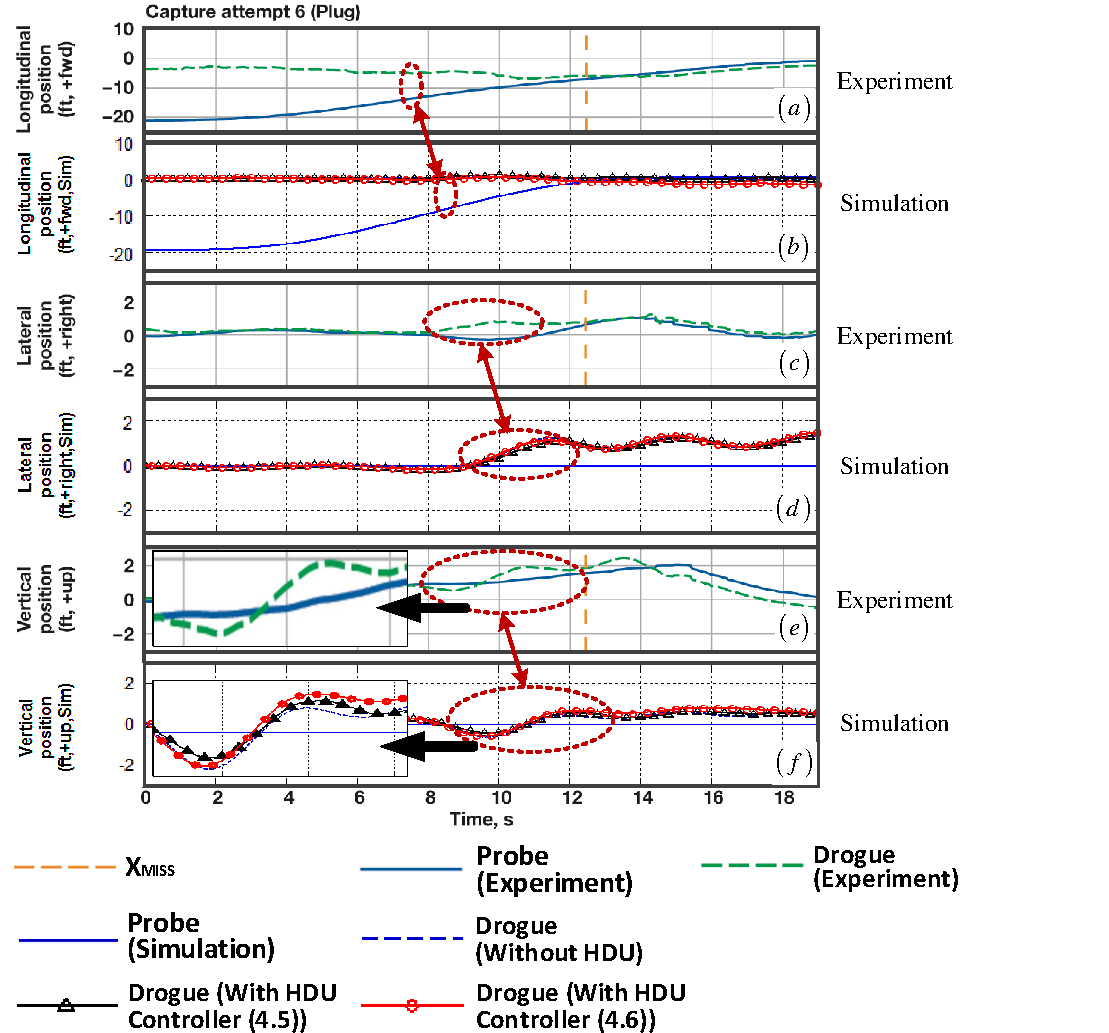
\includegraphics[width=0.7\textwidth]{Figures/Figs_Ch8/Fig12}
	\caption{Comparison of Drogue Dynamics during the Docking Process}\label{F_Comparison}
\end{figure} 
Based on Fig. \ref{F_Comparison}, the HDU has a slight influence on the drogue dynamics. However, during the docking process, even a small error of a few centimeters can lead to docking failure. Therefore, this influence remains significant. The two subplots Fig. \ref{F_Comparison} (e) and (f) illustrate the differences in drogue dynamics in the vertical direction during docking, which is in accordance with the issue highlighted in the conclusions of Section 4.3.
Additionally, from Fig. \ref{F_Sim_Subsidence}, it's even more evident that compared with the scenario without HDU, the vertical descent of the drogue with HDU is significantly reduced. In other words, the drogue dynamics considering the HDU model closely resemble the drogue dynamics observed in experiments.

On the other hand, from Fig. \ref{F_Comparison}, it is evident that the drogue dynamics under the control of the second type of controller differ from those without HDU and those under the control of the first type of controller. Although the swing amplitude of the drogue increases under the second type of controller, its adjustment speed is faster, which is more conducive to suppressing the hose whipping phenomenon. Furthermore, it can lead to a more accurate linearization of the model for the link-connected hose-drogue system with HDU. Therefore, it is still recommended to use the second type of controller for future HDU controller design.
\begin{figure}[th]
	\centering
	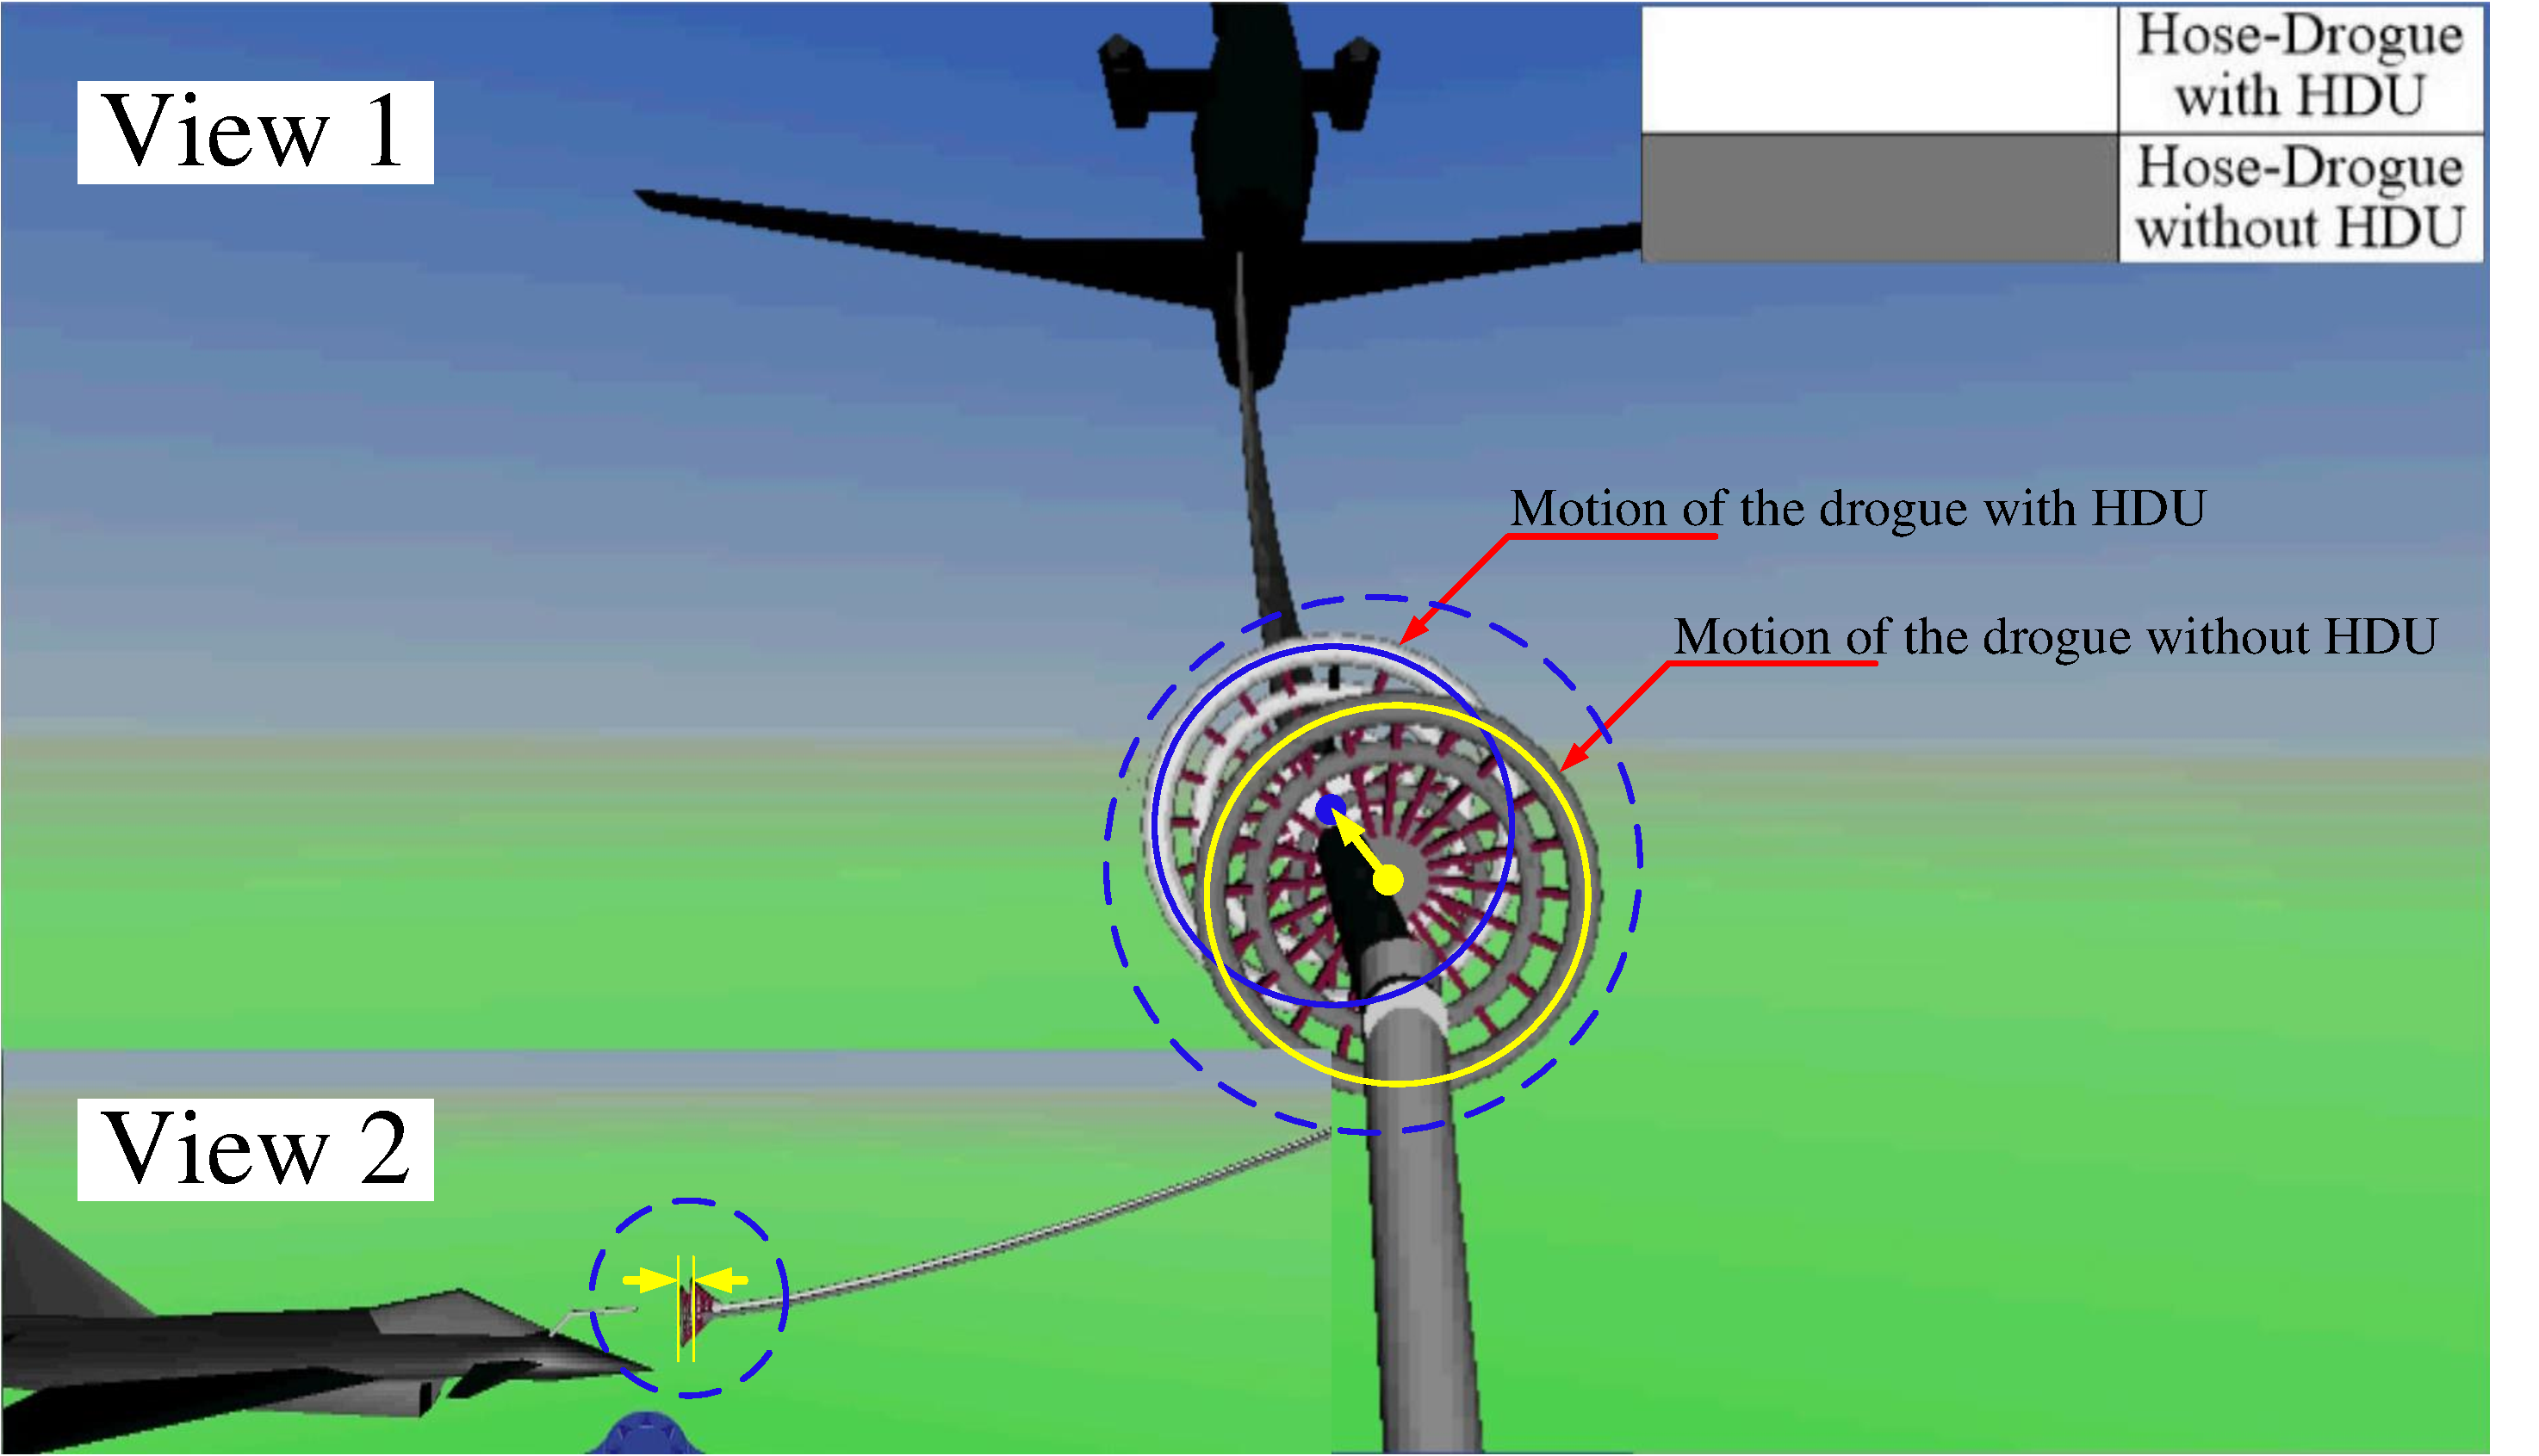
\includegraphics[width=0.7\textwidth]{Figures/Figs_Ch8/Fig13}
	\caption{Screenshot of the Simulation Video at Maximum Drogue Subsidence}\label{F_Sim_Subsidence}
\end{figure} 

\subsection{The Effect of HWP Suppression of Traditional HDU control methods}

In order to estimate the effect that the traditional HDU control methods
suppress the HWP after the excessive contact between the probe and
the drogue, comparison simulations are performed and the results are
shown in Fig.\,\ref{F_Comparison_WAPE}, where an impulse disturbance
(500N$\cdot$s) is injected into the hose-drogue system at 5s to simulate
the excessive contact on the drogue. It can be observed from Fig.\,\ref{F_Comparison_WAPE}
that the hose-drogue system with HDU controller has a larger longitudinal
offset and a smaller vertical offset than those of the hose-drogue
system without HDU controller, where the larger longitudinal offset
is caused by the hose being reeled up by the HDU controller to avoid
vertical offset. The vertical offset indicates that the current HDU
control methods can suppress the HWP to some extent, but the effect
is very limit and it cannot avoid the HWP essentially. In the next
section, a new HDU controller is proposed to avoid the HWP and improve
the safety of probe-and-drogue systems.

\begin{figure}[ptbh]
	\begin{centering}
		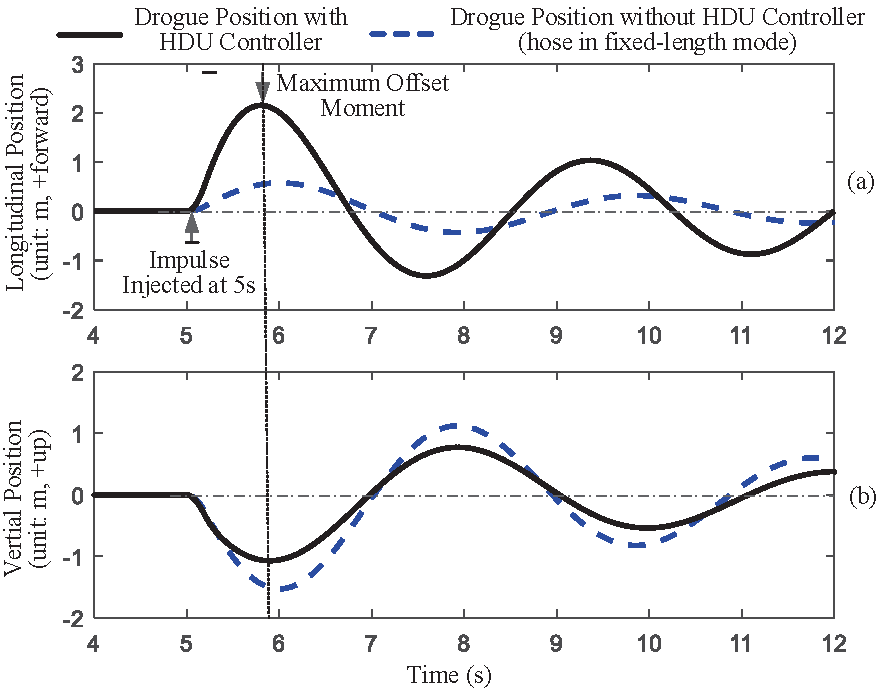
\includegraphics[width=0.48\textwidth]{Figures/Figs_Ch8/Fig14} 
		\par\end{centering}
	\caption{Comparison of motions of the drogue after excessive contact.}
	\label{F_Comparison_WAPE}
\end{figure}

\section{Anti-HWP Control Method for HDU}

The traditional HDU control methods mainly feedback the hose tension
to reduce the drogue fluctuation and suppress HWP to some extent,
but it cannot avoid HWP essentially because it cannot detect whether
the HWP happens. For example, when the probe is docked into the drogue,
it may drive the drogue to continue to move forward a distance, which
may cause the hose slack and reach to a new equilibrium state as shown
in Fig.\,\ref{F_Schematic}(b). In this situation, the hose tension
remains unchanged so the traditional HDU control methods cannot work
correctly, but HWP will happen if the probe accidentally breaks away
from the drogue. Therefore, the HWP is essentially caused by the over-slack
of the hose due to excessive contact on the drogue. In order to avoid
HWP, the HDU controller must be able to observe the hose slack degree
and roll up the hose with an appropriate control method. This section
will present an anti-HWP control method from three aspects: HWP observation,
control method, and simulation verification.

\begin{figure}[ptbh]
	\begin{centering}
		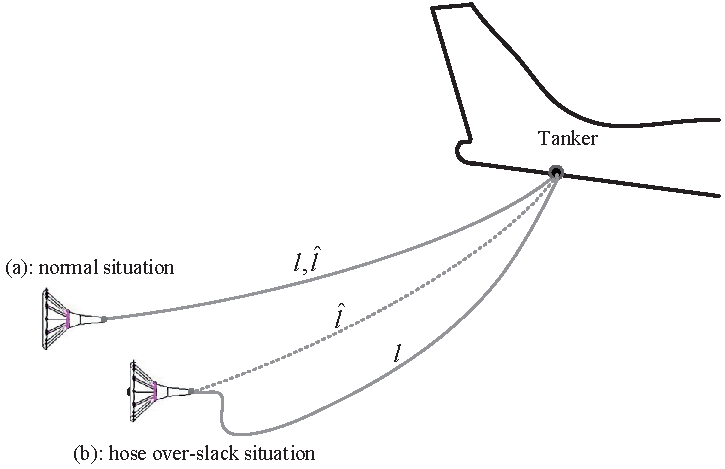
\includegraphics[width=0.48\textwidth]{Figures/Figs_Ch8/Fig15}
		\par\end{centering}
	\caption{Schematic diagram for HWP. The symbol $l$ is the hose length and
		$\hat{l}$ is the desired hose length.}
	\label{F_Schematic}
\end{figure}


\subsection{HWP observation}

\subsubsection{Drogue Position Estimation}

The most direct way to detect HWP is to observe the shape of the hose
through computer vision methods, but it is impractical and unreliable
for real aerial refueling systems. Observing the position of the drogue
$\mathbf{p}_\text{d}$ to estimate the hose slack degree indirectly
for HWP is a more feasible way, which is adopted in this chapter. The
drogue position $\mathbf{p}_\text{d}$ is essential for the docking
control of autonomous aerial refueling system to estimate the relative
position between the probe and the drogue. There are many mature methods
to estimate the drogue position, among which the vision-based methods
\cite{Dibley2007PhaseI,Tandale2008Trajectory} are the
most convenient and widely used one. These methods can be applied to estimate the drogue position for the following HDU control method.


\subsubsection{Hose Slack Degree}

With the drogue position $\mathbf{p}_\text{d}$ and the total hose
length $l$, how to define the hose slack degree and how to estimate
it are presented in this subsection. First of all, the normal situation
with no hose slack is presented as shown in Fig.\,\ref{F_Schematic}(a),
which is the equilibrium state of the hose when the desired hose length
$\hat{l}$ is defined to equal to the hose length $l$, i.e., $l=\hat{l}$.
Second, when the hose is over-slack as presented in Fig.\,\ref{F_Schematic}(b),
the hose length should be larger than its desired value, i.e., $l>\hat{l}$.
Consequently, the hose slack degree $\mu_\text{slack}$ can be defined
as
\begin{equation}
\mu_\text{slack}\triangleq\left|\frac{l-\hat{l}}{\hat{l}}\right|\label{eq:SlackDegree}
\end{equation}
which can be used to describe the hose state and predict the degree
of HWP. The slack degree $\mu_\text{slack}=0$ indicates that the hose
is in the desired state with no over-slack. The more the slack degree
$\mu_\text{slack}$ increases, the more the hose is bent which indicates
a more serious HWP is ready to happen.

In order to obtain $\mu_\text{slack}$, the method to obtain the desired
hose length $\hat{l}$ should be given first. As shown in Fig.\,\ref{F_Schematic}(a),
the desired hose shape is a smooth curve, whose length $\hat{l}$
can be written as a function that depends on the drogue position $\mathbf{p}_{\text{d}}$
as
\begin{equation}
\hat{l}=f_{\hat{l}}\left(\mathbf{p}_{\text{d}}\right)
\end{equation}
where $f_{\hat{l}}\left(\cdot\right)$ can be obtained by hose modeling
methods \cite{Ro2011,Wang2014} or look-up table methods. However,
in practice, the precise expressions of $\hat{l}$ for different flight
conditions (altitude and speed) are very complicated and unobtainable.
Alternatively, an approximate estimation method for $\hat{l}$ is
developed in this chapter. Based on the simulation results with the
hose model \cite{Ro2011,Wang2014}, the estimation expression for
the desired length $\hat{l}$ is approximate to a function of the
straight-line distance of the drogue $\left\Vert \mathbf{p}_{\text{d}}\right\Vert $
as
\begin{equation}
\hat{l}\approx f_{\hat{l}}^{\prime}\left(\left\Vert \mathbf{p}_{\text{d}}\right\Vert \right)\approx\frac{\left\Vert \mathbf{p}_{\text{d}}\right\Vert }{\left\Vert \mathbf{p}_{\text{d}0}\right\Vert }\cdot l_{0}\label{eq:HoseLengthEst}
\end{equation}
where $\mathbf{p}_{\text{d}0}$ and $l_{0}$ are the initial equilibrium
drogue position and hose length. The maximum estimated error $\varepsilon_{\hat{l}}$
for (\ref{eq:HoseLengthEst}) is given by
\begin{equation}
\varepsilon_{\hat{l}}=\max_{\mathbf{p}_{\text{d}}\in\Omega}\frac{\left|\hat{l}-\frac{\left\Vert \mathbf{p}_{\text{d}}\right\Vert }{\left\Vert \mathbf{p}_{\text{d}0}\right\Vert }\cdot l_{0}\right|}{\hat{l}}\label{eq:err}
\end{equation}
where $\Omega$ denotes a safe region for the normal drogue movement.
According to the simulation results, $\varepsilon_{\hat{l}}$ is very
small but still the following anti-HWP control method will well consider
this error and hand it for robustness requirements.

\subsubsection{HWP Detection}

Safety is always the most fundamental requirement for any aerial refueling
system. To avoid the damage of HWP after excessive or abnormal impact
on the drogue, this subsection presents a method to detect the hose
state and classify it into three situations based on its hazardous
degree.

(i) \textbf{Normal Situation}. Ideally, the normal situation should
be $\mu_\text{slack}=0$; namely, the hose coincides exactly with the desired
hose curve as shown in Fig.\,\ref{F_Schematic}(A). However, it is unreachable
in practice due to the estimated error of (\ref{eq:HoseLengthEst})
and other uncertain errors, such as the small fluctuation of the hose
under atmospheric turbulence. Therefore, a minimum slack threshold
$\varepsilon_{\min}$ is defined as shown in Fig.\,\ref{F_Safety}.
The normal situation of the hose is defined by the criterion
\begin{equation}
\mu_\text{slack}\leq\varepsilon_{\min}\text{ and }\mathbf{p}_{\text{d}}\in\Omega\label{eq:AAA}
\end{equation}
where the threshold $\varepsilon_{\min}$ should cover the estimation
error ($\varepsilon_{\min}>\varepsilon_{\hat{l}}$) and other uncertain
errors for robustness requirements. For simplicity, it can be select
as $\varepsilon_{\min}=2\varepsilon_{\hat{l}}$ for a 100\% safe margin.
In (\ref{eq:AAA}), the safe region $\mathbf{p}_{\text{d}}\in\Omega$ is
presented as the meshed region in \ref{F_Safety}. If the drogue
is out of this region ($\mathbf{p}_{\text{d}}\notin\Omega$), it indicates
that an abnormal big swing is already appearing and emergency measures
should be taken immediately.

(ii) \textbf{Over-slack Situation}. The over-slack situation is defined
as that the hose slack degree $\mu_\text{slack}$ is out of ``normal range''
in (\ref{eq:AAA}) and it is within the controllable region for the
HDU controller to safely reduce the slack degree $\mu_\text{slack}$ to
the normal situation. Similar to (\ref{eq:AAA}), the over-slack situation
can be defined by the following criterion
\begin{equation}
\varepsilon_{\min}<\mu_\text{slack}\leq\varepsilon_{\max}\text{ and }\mathbf{p}_{\text{d}}\in\Omega\label{eq:BBB}
\end{equation}
where $\varepsilon_{\max}$ is the maximum slack threshold as shown
in Fig.\,\ref{F_Safety}, which is selected based on the safety
requirement and controller performance.

(iii) \textbf{Unsafe Situation}. The unsafe situation is defined as
the complementary set of (\ref{eq:AAA})(\ref{eq:BBB})
\begin{equation}
\mu_\text{slack}>\varepsilon_{\max}\text{ or }\mathbf{p}_{\text{d}}\notin\Omega.\label{eq:unsafe}
\end{equation}
When the drogue-drogue system reaches this situation, it means that
a serious HWP is happening or ready to happen. To ensure the safety
of the hose-and-drogue system, emergency measures should be applied
immediately. For example, rolling up the hose with maximum speed to
avoid a collision on the receiver aircraft.

For the above three situations, different control strategies will
be adopted to avoid the HWP and ensure the safety of the drogue-hose
system. When the hose is in the normal situation, it indicates that
no impact or abnormal oscillation is happening on the drogue, so the
traditional HDU control methods as presented in Section 8.2
can be applied to reduce the drogue position fluctuation for improving
the docking success rate. When the hose is in the unsafe situation,
emergency control measures should be carried out to avoid further
damage on the receiver aircraft or equipment. For example, HDU controller
rolls up the hose with the maximum speed to leave a safe distance
between the hose and the receiver aircraft. Since the over-slack situation
is the most important stage to handle impact on the drogue and avoid
HWP, the next subsection will focus on the anti-HWP controller design
in this situation.

\begin{figure}[ptbh]
	\begin{centering}
		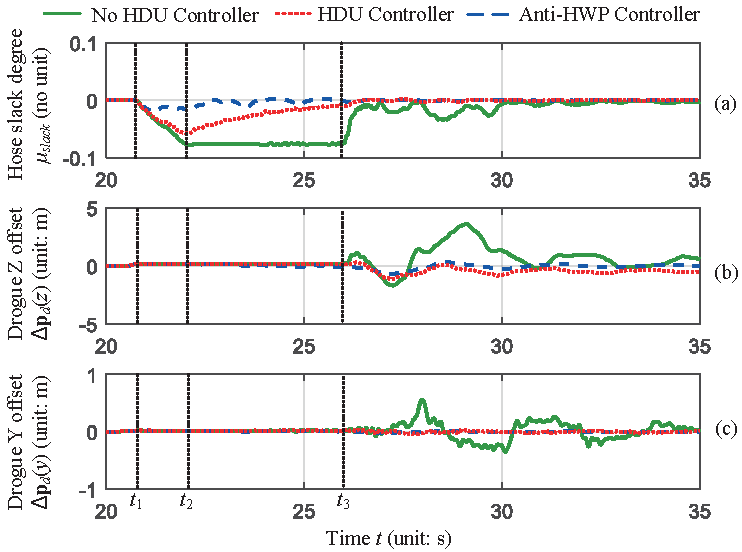
\includegraphics[width=0.48\textwidth]{Figures/Figs_Ch8/Fig16}
		\par\end{centering}
	\caption{Safety criteria for the hose-drogue system.}
	\label{F_Safety}
\end{figure}


\subsection{Anti-HWP Control}

The objective of the anti-HWP controller for HDU is to smoothly control
the hose length to change the hose state from the over-slack situation
($\varepsilon_{\min}<\mu_\text{slack}\leq\varepsilon_{\max}$) to the normal
situation ($\mu_\text{slack}\leq\varepsilon_{\min}$). Then, the traditional
HDU controller is capable of stabilizing the hose-and-drogue system
to an equilibrium state in the normal situation.

First of all, a speed feedback control is given by

\begin{equation}
T_\text{reel}=T_\text{hose}-m_\text{reel}\cdot k_{\text{d}}\cdot\left(\dot{l}-\hat{\dot{l}}\right)\label{eq:ctrl2}
\end{equation}
where $\hat{\dot{l}}$ is an indirect control input signal that indicates
the desired increasing speed of the hose length, and $k_{\text{d}}>0$ is
a controller parameter. Substituting (\ref{eq:ctrl2}) into the HDU
model (\ref{E_HDU1}) gives
\begin{equation}
\ddot{l}=\frac{T_\text{reel}-T_\text{hose}}{m_\text{reel}}=-k_{\text{d}}\cdot\left(\dot{l}-\hat{\dot{l}}\right).\label{eq:Ctrol1}
\end{equation}
which is an exponentially convergent system that ensures the HDU track
the given speed as $\dot{l}\rightarrow\hat{\dot{l}}$. Second, the
desired speed input $\hat{\dot{l}}$ is further given by
\begin{equation}
\hat{\dot{l}}=-k_\text{p}\cdot\left(l-\hat{l}\right)\label{eq:kp}
\end{equation}
where $k_\text{p}>0$ is a controller parameter. Note that, in practice,
a saturation function can be added to (\ref{eq:kp}) to prevent the
drogue from pulling out the probe if the hose rolls up too fast. Finally,
by combining (\ref{eq:HoseLengthEst})(\ref{eq:ctrl2})(\ref{eq:kp}),
the anti-HWP controller can be written as
\begin{equation}
\begin{array}{cl}
T_\text{reel}= & T_\text{hose}+m_\text{reel}k_{\text{d}}k_\text{p}\frac{\left\Vert \mathbf{p}_{\text{d}}\right\Vert }{\left\Vert \mathbf{p}_{\text{d}0}\right\Vert }l_{0}\\
& -m_\text{reel}k_{\text{d}}\cdot\dot{l}-m_\text{reel}k_{\text{d}}k_\text{p}\cdot l
\end{array}.\label{eq:CTRL1}
\end{equation}
The following theorem provides the convergence condition under which
one can conclude the convergence property of the designed TILC controller
in (\ref{eq:CTRL1}).

\textbf{Theorem 1}. Consider a hose-and-drogue system with the HDU
structure described by (\ref{E_ModelHDU})(\ref{E_HDU1}). Suppose
(i) the hose state is in over-slack situation (\ref{eq:BBB}); (ii)
the anti-HWP controller is designed as (\ref{eq:CTRL1}) with its
parameters satisfy
\begin{equation}
k_\text{p}>0,k_{\text{d}}>0
\end{equation}
Then, the hose slack degree $\mu_\text{slack}$ can converge to zero, i.e.,
$\mu_\text{slack}\left(t\right)\rightarrow0$.

\textbf{Proof.} Combining (\ref{eq:Ctrol1})(\ref{eq:kp}) gives
\begin{equation}
\ddot{l}+k_{\text{d}}\dot{l}+k_{\text{d}}k_\text{p}\left(l-\hat{l}\right)=0.\label{eq:sss}
\end{equation}
By letting $\Delta l\triangleq l-\hat{l}$, for constant value $\hat{l}$,
(\ref{eq:sss}) can be rewritten as

\begin{equation}
\Delta\ddot{l}+k_{\text{d}}\Delta\dot{l}+k_{\text{d}}k_\text{p}\Delta l=0.\label{eq:qq}
\end{equation}
It can be observed from (\ref{eq:qq}) that controller (\ref{eq:CTRL1})
is essentially a PD (Proportion Differentiation) controller with proportion
coefficient $k_\text{p}$ and differentiation coefficient $k_{\text{d}}$. Therefore,
(\ref{eq:qq}) is a stable second-order linear system when $k_{\text{d}}>0$
and $k_{\text{d}}>0$, which will converge exponentially to zero
\begin{equation}
\lim_{t\rightarrow\infty}\left|l\left(t\right)-\hat{l}\right|=\lim_{t\rightarrow\infty}\left|\Delta l\left(t\right)\right|=0.\label{eq:conv}
\end{equation}
Then, according to the definition of $\mu_\text{slack}$ in (\ref{eq:SlackDegree}),
it can be derived from (\ref{eq:conv}) that
\begin{equation}
\mu_\text{slack}\left(t\right)\triangleq\left|\frac{l\left(t\right)-\hat{l}}{\hat{l}}\right|=\frac{\left|\Delta l\left(t\right)\right|}{\hat{l}}\rightarrow0\label{eq:aaa}
\end{equation}
which indicates that the hose slack degree $\mu_\text{slack}$ can converge
to zero under controller (\ref{eq:CTRL1}). $\Square$

According to \textit{Theorem 1}, when the hose slack degree is in
the range $\varepsilon_{\min}<\mu_\text{slack}\leq\varepsilon_{\max}$,
it will always converge to zero, which means the slack degree can
eventually be reduced into region $\mu_\text{slack}\leq\varepsilon_{\min}$.
Then, the traditional HDU controller will take over the control privilege.
According to research in \cite{dai2018terminal}, the hose-and-drogue
system is a self-stabilizing system, and it will be stabilized to
an equilibrium state under the effect of gravity, air drag and air
viscous.

\subsection{Simulation Verification}

A series of simulations are performed to verify the effect of the
proposed anti-HWP controller. The basic parameters are listed in Table
\ref{T_SimEnvironment}, and additional parameters are given below
\[
\varepsilon_{\min}=0.004,\varepsilon_{\max}=0.05,k_{\text{d}}=10,k_\text{p}=3.
\]
The variable length hose-drogue model \cite{Wang2014} with the link
number $N=20$ is used in these simulations for better simulation
accuracy and display effect. A video has also been released to introduce
the simulation environment and demonstrate the control effect of the
proposed anti-HWP controller method. The URL of the video is \url{https://youtu.be/s9XgGICqKtA}.

\begin{figure}[ptbh]
	\begin{centering}
		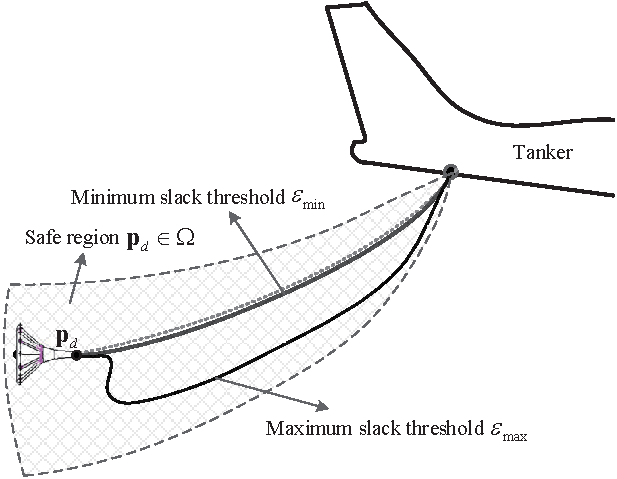
\includegraphics[width=0.48\textwidth]{Figures/Figs_Ch8/Fig17}
		\par\end{centering}
	\caption{Simulations of probe-and-drogue system with and without anti-HWP controller.}
	\label{F_Sim_HWP}
\end{figure}

Fig.\,\ref{F_Sim_HWP} presents three typical comparative simulation
results: 1) the simulation results (solid green curves in Fig.\,\ref{F_Sim_HWP})
with no HDU controller, where the HDU controller is not enabled, and
the hose length remains unchanged during the whole simulation; 2)
the simulation results (dotted red curves in Fig.\,\ref{F_Sim_HWP})
with the existing HDU control method, where the HDU controller is
enabled to control the hose length to weaken HWP; 3) the simulation
results (dash blue curves in Fig.\,\ref{F_Sim_HWP}) with the proposed
anti-HWP method, where the anti-HWP controller is enabled to control
the hose length to avoid HWP safely. The above three simulations all
contain the following stages: (i) the receiver flies close to the
drogue from time $0\text{s}\sim t_{1}$; (ii) the contact between
the probe and the drogue happens at $t_{1}$; (iii) the probe drives
the drogue fly forward a distance from time $t_{1}\sim t_{2}$; (iv)
the probe holds the drogue and remains relatively static from time
$t_{2}\sim t_{3}$; (v) the receiver suddenly breaks away from drogue
at time $t_{3}$ and flies backward from time $t_{3}\sim35\text{s}$.

It can be observed from Fig.\,\ref{F_Sim_HWP}(a): 1) the hose
slack degree increase to a large for simulation curve with no HDU
controller, which indicates a serious HWP is happening; 2) the hose
slack degree increase to a medium value for simulation curve with
an HDU controller but its slack degree is much smaller than the simulation
curve with no HDU controller, which indicates that the existing HDU
control methods can suppress HWP but cannot completely avoid it; 3)
there is almost no hose slack for simulation curve with anti-HWP controller,
which indicates the HWP is successfully avoided. Figs.\,\ref{F_HWPVR}(a)(b)
show the slack states of the hose with no HDU controller and with
the proposed anti-HWP controller. Due to the over-slack state of the
hose, a significant HWP is observed in the simulation without the
anti-HWP controller, which is reflected in the drastic position fluctuation
along Y and Z directions in Fig.\,\ref{F_Sim_HWP}(b)(c). By contrast,
the hose and drogue states are both very steady with the proposed
anti-HWP controller, and no HWP happens as expected. The above results
indicate that, compared with the existing HDU control methods, the
proposed anti-HWP control method can effectively avoid the HWP and
ensure the safety of hose-and-drogue systems.

\begin{figure}[ptbh]
	\begin{centering}
		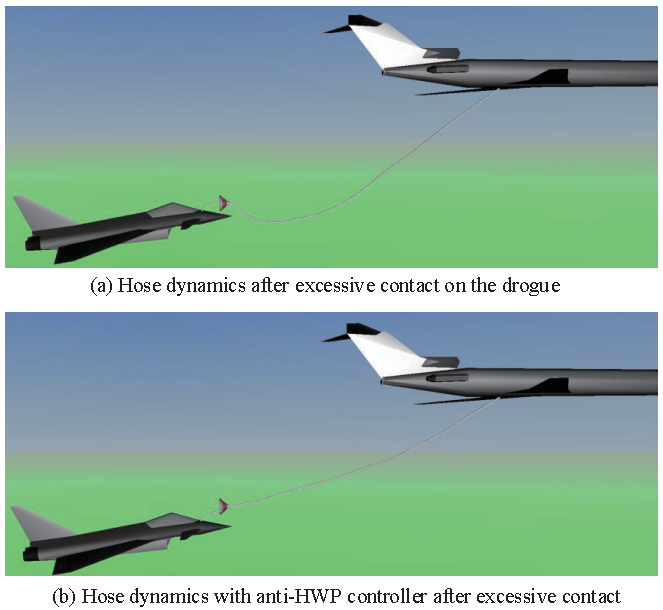
\includegraphics[width=0.48\textwidth]{Figures/Figs_Ch8/Fig18}
		\par\end{centering}
	\caption{Visual display of the hose-and-drogue systems under excessive contact.}
	\label{F_HWPVR}
\end{figure}


\section{Chapter Summary}

It is critical to analyze the dynamics of the drogue under the bow
wave, for designing docking controllers and docking simulations. However,
this problem is not considered comprehensively in the existing literature.
This chapter integrates the HDU model, the bow wave model and the variable
length hose-drogue model into an integrated model. Then, two types
of controllers are designed for HDU. One type is the commonly used
controller used in the real PDR, and the other one is an improved
one based on the commonly used controller. Based on the integrated
model, the drogue dynamic models under different HDU controllers are
obtained through system identification, and the performance of them
are analyzed. By considering the effects of HDU, the dynamics of the
proposed method is in better agreement with the real experiment than
our previous study. Meanwhile, the traditional HDU control methods
mainly feedback the hose tension to reduce the drogue fluctuation
and suppress HWP to some extent, but it cannot avoid HWP essentially.
An anti-HWP control method is proposed to significantly reduce the
effect of the hose whipping phenomenon and improve the safety of aerial
refueling systems. Finally, the effectiveness of the proposed modeling
method and the anti-HWP control method are well verified by simulations
and comparisons.